\documentclass[12pt]{article}

\usepackage{blindtext} % Package to generate dummy text throughout this template 
\usepackage{amssymb, amsthm, amsmath}

% writing
\usepackage[utf8]{inputenc}
\usepackage{algorithm}
\usepackage[noend]{algpseudocode}
\linespread{1.5}
\usepackage[margin = 1in]{geometry}
\usepackage{microtype} % Slightly tweak font spacing for aesthetics
\usepackage[english]{babel} % Language hyphenation and typographical rules

% tikz
\usepackage{tikz}
\usepackage{pgfplots}
%\usepackage{pgfplotstable}
\pgfplotsset{compat=1.13}
\usetikzlibrary{external}
\tikzexternalize[prefix=external-figures/]

% fig
\usepackage{natbib}
\usepackage{graphicx}
\usepackage{float}
\usepackage{wrapfig}
\usepackage{multicol}

% misc
\usepackage{nomencl}
\usepackage[titletoc, page]{appendix}
\usepackage{multirow}

% caption features
\usepackage{caption}
\usepackage{subcaption}
\usepackage{setspace}
\captionsetup{font={small, stretch=1.25}}
\let\Algorithm\algorithm
\renewcommand\algorithm[1][]{\Algorithm[#1]\setstretch{1.25}}

% ref
\usepackage[pdfpagelabels]{hyperref}
\usepackage{url}
\hypersetup{
    colorlinks=true,
    linkcolor=black,
    urlcolor=black,
    citecolor=black
}
\usepackage[capitalise]{cleveref}
\crefname{appsec}{Appendix}{Appendices}
%\Crefformat{section}{\S#2#1#3}
%\Crefformat{subsection}{\S#2#1#3}
%\Crefformat{subsubsection}{\S#2#1#3}

\setlength{\parindent}{2em}
%\setlength{\parskip}{1.5em}
\graphicspath{ {images/} }

% nomenclature specs
\makenomenclature
\setlength{\nomitemsep}{-\parsep}
\renewcommand{\nomname}{List of Functions, Symbols and Terms}
%% This code creates the groups
% -----------------------------------------
\usepackage{etoolbox}
\renewcommand{\nomgroup}[1]{%
    \item[\bfseries
    \ifstrequal{#1}{T}{Terms}{%
        \ifstrequal{#1}{S}{Symbols}{%
            \ifstrequal{#1}{F}{Functions}{}}%
    }]}
% -----------------------------------------

\newtheorem{mydef}{Definition}
\newcommand{\vect}[1]{\mathbf{#1}}  % vector
\newcommand{\matr}[1]{\mathbf{#1}}  % matrix
\newcommand{\tens}[1]{\mathbf{#1}}  % tensor
\newcommand{\mean}[1]{\overline{#1}}    % mean overline

\title{Report: Solving the Avicaching Problem Faster and Better}
\author{Anmol Kabra, Yexiang Xue and Carla Gomes}
\date{Summer 2017}

\begin{document}
    \pagenumbering{roman}
\begin{titlepage}
    \maketitle
    \thispagestyle{empty}
\end{titlepage}

% nomenclature
\mbox{}
% symbols
\nomenclature[S]{$J$}{Number of locations in the dataset}
\nomenclature[S]{$T$}{Number of time units for which data is available}
\nomenclature[S]{$n_F$}{Number of features in the dataset $\matr{F}$ (length of $\matr{F}[v][u]$)}

% functions
\nomenclature[F]{softmax($\cdot$)}{Defined as softmax($z_i$) = $\frac{\exp(z_i)}{\sum_{i} \exp(z_i)}$}
\nomenclature[F]{reLU($\cdot$)}{Rectified Linear Unit; defined as reLU($z$) = max(0, $z$)}
\nomenclature[F]{batch-multiply($\cdot$)}{Operates on $m \times n \times p$ and $m \times p \times q$ tensors to give a $m \times n \times q$ tensor.}
\nomenclature[F]{$\matr{A} \cdot \matr{B}$}{(dot product) Defined as $\matr{A}\matr{B}^T$ as per convention}

% terms
\nomenclature[T]{Epoch}{One training/testing period; iteration}
\nomenclature[T]{CPU ``set''}{\textit{All} operations done on the CPU}
\nomenclature[T]{GPU ``set''}{\textit{Only Matrix/Tensor} operations done on the GPU, rest on the CPU}
\nomenclature[T]{LP}{Linear Programming}
\nomenclature[T]{LP Standard Format}{Arrangement of objective function and constraints operated on by library LP solvers - minimize [$\vect{c}^T \vect{x}$]; subject to [$\matr{A} \vect{x} \leq \vect{b}, \, x_i \geq 0$]}
\nomenclature[T]{Tensor}{Multi-dimensional (usually more than 2 dimensions) array}
\printnomenclature[1.5in]

\tableofcontents
%\listoftables
%\listoffigures
\cleardoublepage
\pagenumbering{arabic}
    
    % main body
    \chapter{Introduction} \label{sec:Introduction}
Optimizing predictive models on datasets obtained from citizen-science projects can be computationally expensive as these datasets grow in size. Consequently, running models based on Multi-layered Neural Networks, Integer Programming and other optimization routines can become more computationally difficult as the number of parameters increase, despite using the faster Central Processing Units (CPUs) in the market. Incidentally, it becomes difficult for citizen-science projects, which often deal with large datasets, to scale if the organizers do not employ special processing units to run neural networks as optimization models, which require extensive tensor operations. One such special processing unit is the Graphical Processing Units (GPUs), which offer numerous cores to parallelize computation. These can often outperform CPUs in computing such predictive models if these models \textit{heavily} rely on large-scale tensor operations \cite{ParallelNVIDIA, cuDNNPaper}. By using GPUs over CPUs to accelerate computation on a citizen-science project, the model could achieve better optimization in less time, enabling the project to scale.

\section{Avicaching} \label{sec:Avicaching}
Part of the eBird project, which aims to ``maximize the utility and accessibility of the vast numbers of bird observations made each year by recreational and professional bird watchers'' \cite{EBird}, Avicaching is a incentive-driven game trying to homogenize the spatial distribution of citizens' (agents') observations \cite{Xue2016Avi1, Xue2016Avi2}. Since the dataset of agents' observations in eBird is geographically heterogeneous (concentrated in some places like cities and sparse in others), Avicaching homogenizes the observation set by placing rewards at and attracting agents to under-sampled locations \cite{Xue2016Avi1}. For the agents, collecting rewards increases their `utility' (excitement, fun etc.), while for the organizers, a more homogeneous observation dataset means better sampling and higher confidence in using it for other models. 
\begin{figure}[!htbp]
    \centering
    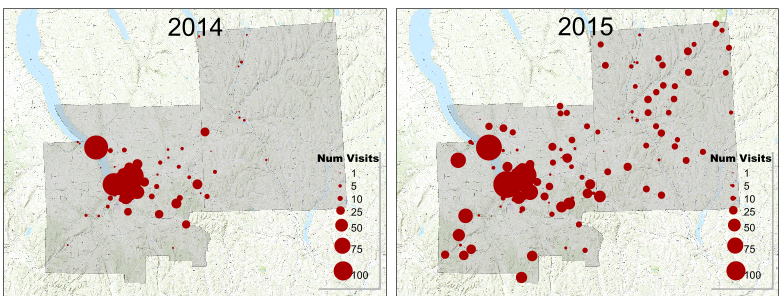
\includegraphics[width=\textwidth]{avicaching_change}
    \caption[Avicaching 2014-15 Results in Tompkins and Cortland Counties]{Avicaching 2014-15 Results in Tompkins and Cortland Counties, NY: With the previous model \cite{Xue2016Avi1, Xue2016Avi2, EBird}, Avicaching was able to attract `eBirders' to under-sampled locations by distributing rewards over the location set.}
    \label{fig:Avicaching 2014-15 Results in Tompkins and Cortland Counties}
\end{figure}

To accomplish this task of specifying rewards at different locations based on the historical records of observations, Avicaching would learn how agents change their behavior when a certain sample of rewards were applied to the set of locations, and then redistribute rewards across the locations based on those learned parameters \cite{Xue2016Avi2}. This requirement naturally translates into a  optimization problem, implemented using multi-layered neural networks and linear programming.

\section{Important Questions} \label{sec:Important Questions}
Although the previously devised solutions to Avicaching were conceptually effective \cite{Xue2016Avi1, Xue2016Avi2}, using CPUs to solve Mixed Integer Programming and (even) shallow neural networks made the models impractical to scale. Solving the problems faster would have also allowed organizers to find better results (more optimized). These concerns, which form the pivot for our research, are concisely described below.

\subsection{Solving Faster} \label{sec:Important Questions - Solving Faster}
We were interested in using GPUs to run our optimization models because of their capability to accelerate problems based on large tensor operations \cite{ParallelNVIDIA, cuDNNPaper}. Newer generation NVIDIA GPUs, equipped with thousands of CUDA (NVIDIA's parallel computing API) cores \cite{NVIDIA}, could have empowered Avicaching's organizers to scale the game, if the underlying models were computed using simple arithmetic operations on tensors, rather than using conditional logic (see~\Cref{sec:Avoiding Specific Operations in GPUs}). Since even the faster CPUs - in the range of Intel Core i7 chipsets - are sequential in processing and do not provide as comparable parallel processing\footnote{CPUs often have multiple cores nowadays, but very few compared to what many GPUs have.} as GPUs do, we sought to solve the problem much faster using GPUs. But \textbf{how fast could we do it?}

\subsection{Better Results} \label{sec:Important Questions - Better Results}
The previously devised sub-model for learning parameters in agents' change of behavior on a fixed set of rewards delivered predictions that differed $26\%$ from Ground Truth \cite[Table~1]{Xue2016Avi2}. This model was then used to redistribute rewards in a budget. If we could get closer to the Ground Truth, i.e., better learn the parameters for the change, we could redistribute rewards with superior prediction/accuracy. Since the organizers require the \textit{best} distribution of rewards, we will need a set of learned parameters that is closer to the Ground Truth (in terms of Normalized Mean Squared Error \cite[Section~4.2]{Xue2016Avi2}). In a gist, we aimed to \textbf{learn the parameters more suitably}, and \textbf{find the  best allocation of rewards.}

\subsection{Adjusting the Model's Features} \label{sec:Important Questions - Adjusting the Model's Features}
Once the model starts delivering better results than the previously devised models, one thinks if some characteristics\footnote{Tinkering with hyper-parameters like learning rate or adding a weight regularizer.} of the model can be changed to get more preferable results (one could also build a better model). While a goal of ``getting better results'' is an unending struggle, there is a trade-off with practicality as these adjustments take time and computation power to test - and we didn't have unlimited resources. Therefore, we asked if one could \textbf{reasonably adjust the model's features to improve performance and optimization.}

\section{Computation Using GPUs} \label{sec:Computation Using GPUs}
The use of GPUs has changed drastically in the last decade - from rendering superior graphics to parallelizing floating point operations. Companies like NVIDIA are now providing General Purpose GPUs (GPGPUs) that are capable of executing parallel algorithms using thousands of cores and threads \cite{NVIDIA}. Furthermore, by working with newly-developed parallel programming APIs like CUDA, one can handle a GPU's threads more efficiently and optimize an task's datapath \cite{CUDADocs}. In the next sections, we briefly describe NVIDIA GPU's architecture, instruction set and best practices for optimization. Although we do not implement the CUDA back-end manually and use PyTorch's implementation \cite{PTDocs}, understanding the basics of the processor can be helpful for designing our models.

\subsection{GPU Architecture} \label{sec:GPU Architecture}
We describe the structure and abstractions of an NVIDIA GPU with Pascal architecture\footnote{We use NVIDIA Quadro P4000 (Pascal architecture) for our tests.}. These devices are multi-threaded multi-processors for executing ``fine-grained threads efficiently'' \cite[Appendix~B.4]{PattersonARM}. Unlike Personal Computer CPUs, which currently comprise 1-8 cores with fast and low-latency datapath, GPUs provide scalable parallel processing power with high throughput and latency\footnote{High latency is undesirable.} \cite{PattersonARM, DemystifyingGPU}. Informally, GPUs are often referred to as a collection of many `dumb' cores, unlike the few `smart' cores in a CPU. Nonetheless, GPUs are efficient in executing simple instructions in parallel, using hierarchies of cores, threads and memory.

\subsubsection{Core Organization}
In most architectures by NVIDIA, many Scalar Processors (SP or CUDA cores) are clustered in a Streaming Multiprocessor (SM), which are then organized in Grid Processing Clusters (GPCs). A GPU can have several GPCs, as shown in \Cref{fig:Organization of Cores in NVIDIA Pascal GP100 GPU} \cite{CUDADocs, ParallelNVIDIA, DemystifyingGPU}.
\begin{figure}
    \centering
    \begin{subfigure}{\textwidth}
        \centering
        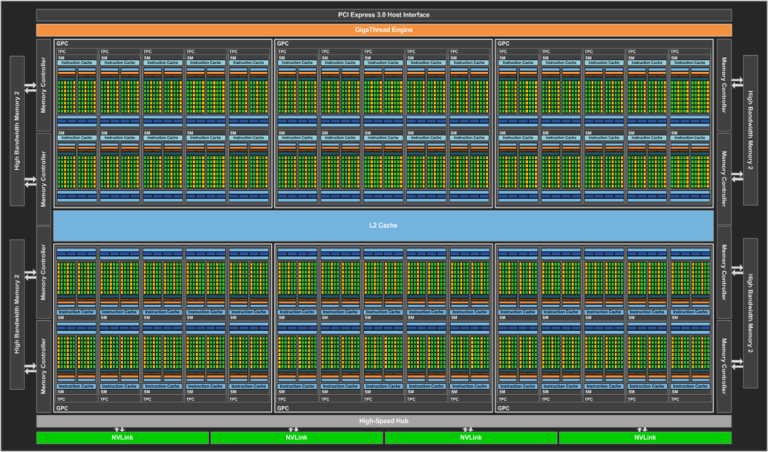
\includegraphics[width=\textwidth]{gpu_pascal}
        \caption[Organization of Cores in NVIDIA Pascal GP100 GPU]{Organization of Cores in NVIDIA Pascal GP100 GPU: In 6 GPCs and 60 SMs, 3840 SP or CUDA Cores (depicted by green blocks) are arranged \cite{PascalWhitepaper, ParallelNVIDIA}.}
        \label{fig:Organization of Cores in NVIDIA Pascal GP100 GPU}
    \end{subfigure}\vspace*{1em}
    \begin{subfigure}{\textwidth}
        \centering
        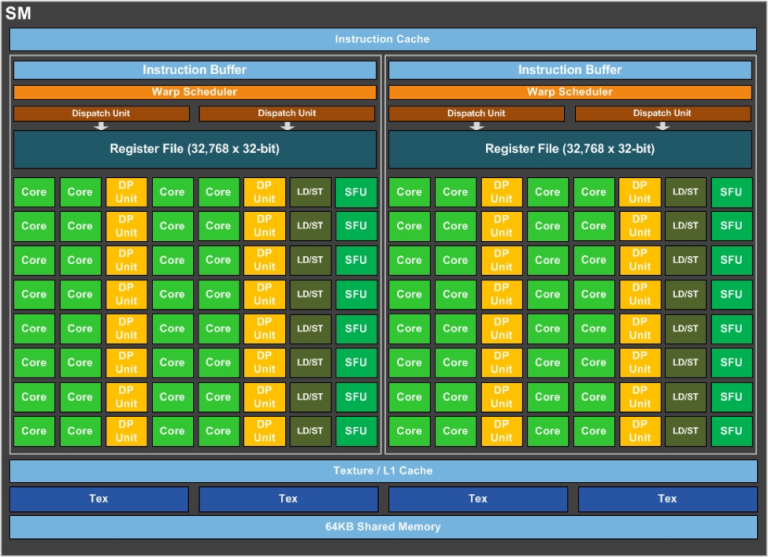
\includegraphics[width=.7\textwidth]{gpu_pascal_sm}
        \caption[Constituents of a Streaming Multiprocessor]{Constituents of a Streaming Multiprocessor \cite{PascalWhitepaper, ParallelNVIDIA}.}
        \label{fig:Constituents of a Streaming Multiprocessor}
    \end{subfigure}
    \caption[The NVIDIA Pascal Architecture]{The NVIDIA Pascal Architecture: A GPU, like a typical CPU, contains multiple hierarchies of memory. In addition, NVIDIA also builds a hierarchy of core organization.}
    \label{fig:The NVIDIA Pascal Architecture}
\end{figure}

The Streaming Multiprocessor (\Cref{fig:Constituents of a Streaming Multiprocessor}), which is the primary multi-threaded multi-processor, houses a shared memory unit for all SPs along with registers and Special Function Units (SFUs), which can calculate specific mathematical functions in fewer clock cycles than threads. The SM is responsible for relaying instructions to threads (in SPs) and maintaining synchronized parallel computation \cite{PascalWhitepaper, DemystifyingGPU}. GPCs and other hierarchies provide abstractions to memory access.

\subsubsection{Memory Organization}
Even the memory units are organized into hierarchies like multi-level caches in CPUs (\Cref{fig:The NVIDIA Pascal Architecture}). In a SM, there are: dedicated local memory units for threads, register files shared by several SPs in a SM, and shared memory units for all SP Cores in a SM \cite{PascalWhitepaper, ParallelNVIDIA}.

The global internal memory of the GPU (like the RAM of a computer), which is housed separately around the clusters of SMs, stores the datasets for a program. Data is then distributed in the shared and local memory units once threads start executing an instruction \cite[Appendix~B]{PattersonARM}. Moreover, similar to the multi-level cache structure in CPUs, GPUs may also have on-chip cache hierarchy (\Cref{fig:The NVIDIA Pascal Architecture}), which enables threads to quickly access working data, thus increasing the performance. On a side note, GPUs' caches are often not big enough to hold full datasets as programs' often require large datasets, leading to more miss rates than caches in CPUs \cite[Appendix~B]{PattersonARM}. 

\subsubsection{Thread Organization}
According to NVIDIA, the parallel structure is obtained by organizing threads into a hierarchy (``grids'' of ``blocks'' of ``warps'' of ``threads''), where threads of a warp (an abstraction) execute in tandem per clock cycle \cite{CUDADocs, DemystifyingGPU}\cite[Appendix~B]{PattersonARM}. In other words, warps are the basic units of execution in a GPU, which receive single instructions from the controller, and forward them to their constituent threads for execution \cite{CUDADocs, DemystifyingGPU}. This abstraction allows the GPU to execute independent sub-tasks in parallel on a large scale(\Cref{fig:GPU - Thread Organization in a GPU}), reducing the total runtime of the program.
\begin{figure}[!htbp]
    \centering
    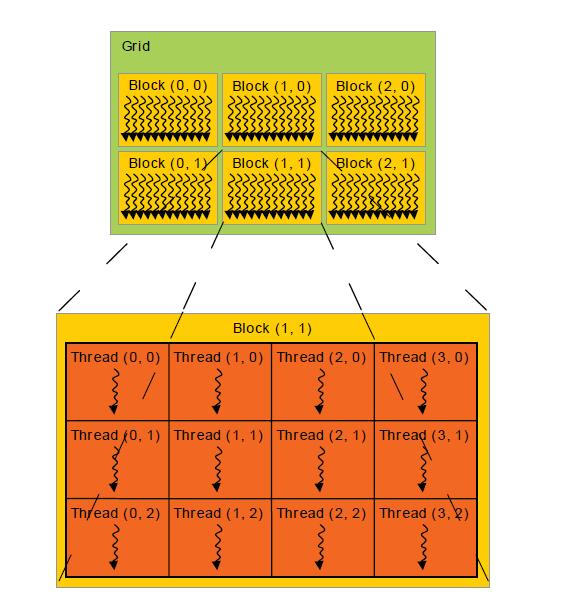
\includegraphics[width=.55\textwidth]{gpu_threads_blocks}
    \caption[Thread Organization in a GPU]{Thread Organization in a GPU: Warps are only an abstraction for identifying threads executing a single instruction; however, threads are physically organized into blocks and grids \cite{CUDADocs,ParallelNVIDIA}}
    \label{fig:GPU - Thread Organization in a GPU}
\end{figure}

NVIDIA calls this setup ``Single-Instruction Multiple-Thread (SIMT)'' \cite{CUDADocs} \cite[Appendix~B.4]{PattersonARM}, where a single instruction is executed in lockstep by multiple threads in a warp (though allowed to branch and diverge). The differences between SIMT and Single-Instruction Multiple-Data (SIMD), a common feature in CPUs, are very subtle. While SIMD distributes data sequences into vectors to be executed by a single core/thread of the CPU (data-level parallelism), SIMT requires a particular thread to only operate on a scalar element of the dataset  \cite{PattersonARM}. In this way, having thousands of threads running in locksteps provides better throughput than doing vector operations per clock cycle. SIMT also allows programmers to write a program meant for a single, independent thread instead of managing vectors in their code, which promotes ease of use and programming \cite[Chapter~4]{CUDADocs}.

\subsubsection{Instruction Set}
The Instruction Set of a GPU is limited, which causes complex instructions to take several clock cycles. Even though a Special Functional Unit (SFU) computes complex functions (transcendental, reciprocal functions) in fewer clock cycles, their number is small compared to the commonplace threads \cite[Appendix~B]{PattersonARM}. The instruction set for Pascal architecture contains basic operations to load and store memory, perform basic floating point and integer (add, subtract, multiply, divide, min, max, left-shift etc.) and binary logical operations (or, and, xor etc.), and execute jump and branching \cite{CUDABinUtils, DemystifyingGPU}. This comprises a very basic set of instructions unlike those in Intel CPUs, for example, which have coalesced and dedicated architecture for complex instructions\footnote{Intel x86 CPUs have Complex Instruction Set Computer (CISC) Design.} \cite{PattersonARM}.

\subsection{Avoiding Specific Types of Operations in GPUs} \label{sec:Avoiding Specific Operations in GPUs}
GPUs are not better than CPUs at many operations, unlike popular perception. With parallel processing comes concerns of synchronization delays, blocking instructions, program correctness etc.. Moreover, since GPUs are separate units of processors, usually connected to CPUs by PCIe lanes, back and forth memory transfer can cause slowdowns in overall performance. Even the GPUs low-level caches are not big enough to deliver hit rates as compared to CPUs. Often there exists a tradeoff when programming with GPUs, and one should take care to avoid such delays.

\subsubsection{Branch and Diverge}
Since NVIDIA GPUs deal with program correctness through inter-block barrier synchronization (synchronizing blocks of threads after some executed instructions), threads can often go out of sync, delaying the next instruction \cite[Appendix~B]{PattersonARM}. This ultimately causes latency due to synchronization, which can aggregate and slowdown the performance of the program.

To avoid such delays and maximize throughput, one should elude from using extensive branching in the program. Using conditional checks can change a thread's datapath, which can possibly block other threads from proceeding at synchronization barriers. This behavior is informally referred to as `branch and diverge' (\Cref{fig:Decrease in GPU Throughput due to Branch and Diverge}), which occurs when some threads in a warp follow a different datapath due to conditional branching, `diverging' from the group. Now when the warp's threads are forced to converge, those diverging threads would take longer to complete the instruction, causing the non-diverging threads to wait. This radically decreases the throughput of the warp, which again diverges from the block, adding up the latency \cite[Appendix~B]{PattersonARM}\cite{DemystifyingGPU}.
\begin{figure}[!htbp]
    \centering
    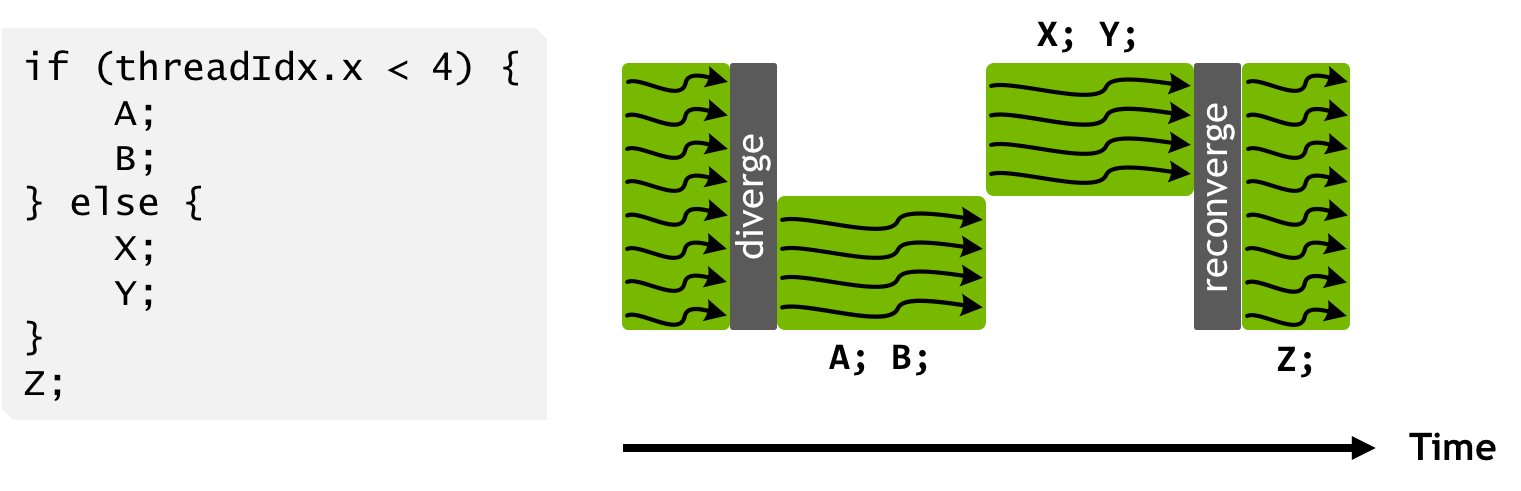
\includegraphics[width=\textwidth]{gpu_branch_diverge}
    \caption[Decrease in GPU Throughput due to Branch and Diverge]{Decrease in GPU Throughput due to Branch and Diverge: In this case, while some threads execute \texttt{A, B}, others execute \texttt{X, Y}. If those sets of operations take unequal time, the threads could diverge from the group and decrease the throughput \cite{ParallelNVIDIA}.}
    \label{fig:Decrease in GPU Throughput due to Branch and Diverge}
\end{figure}

\subsubsection{Memory Limitations}
PCIe lanes are not as fast as on-chip cache access or even RAM access times \cite{CUDADocs, ParallelNVIDIA}. As one would expect, transferring datasets back and forth between GPUs and CPUs can add up considerably. Often the limits of GPU's internal memory or required operations on a dedicated device can force the user to transfer datasets multiple times. Even so, one should look for optimizations that can reduce the number of transfers whenever possible, especially when large datasets are involved.

This suggestion is also applicable when transferring datasets in memory intra-GPU (between caches). Miss rates in a GPU's local caches are often high due to limited size, and data requests from higher-level caches can often be expensive.

\subsection{GPUs' Strengths} \label{sec:Gpu's Strengths}
Inferring from GPUs' weaknesses and architecture, we can say that GPUs are good at handling independent sub-tasks with less diverging sections. These independent sub-tasks can usually be clubbed into matrices and tensors, which the threads operate on in parallel. The fewer conditional branching we have in our algorithms, the better, maintaining the synchronization throughout execution.

Therefore, GPUs are particularly good at doing linear algebra \cite{PattersonARM, ParallelNVIDIA} since most arithmetic operations on matrix elements can be independently solved without branching. Avoiding branching often requires extensive dataset preprocessing; consequently, one should meticulously design the structure of the models' datasets. Tensor-based datasets are often required in machine learning problems, graphics rendering routines, graph-based algorithms etc., which GPUs can potentially accelerate \cite{PattersonARM}.
    \chapter{Problem Formulation} \label{sec:Problem Formulation}
Our models strongly draws from the previous studies \cite{Xue2016Avi1, Xue2016Avi2}, with modifications directed at reducing computation time, as well as getting better results. Since GPUs enable faster computation on tensors, both the Identification and the Pricing Problem are formulated as tensor-based 3-layered and 2-layered neural networks respectively using the Pytorch library \cite{PTDocs}. Recognizing that NVIDIA GPUs easily pair with Pytorch \cite{PTDocs}, accelerating tensor operations using CUDA and cuDNN \cite{cuDNNPaper, NVIDIA}, we aim to maximize parallel operations and minimize thread synchronization.

\section{Identification Problem} \label{sec:Identification Problem}
As discussed in \Cref{sec:Introduction}, the model should learn parameters that caused the change in agents' behavior when a certain set of rewards was applied to locations in the experiment region. Learning those parameters will help us understand how agents behave with a fixed reward distribution, and will enable organizers to redistribute rewards based on that behavior.

Specifically, given datasets $\vect{y_t}$ and $\vect{x_t}$ of agents' visit densities at time $t$, before and after the rewards $\vect{r_t}$ were placed, we want to find weights $\matr{w_1}$ and $\matr{w_2}$ that caused the change from $\vect{x_t}$ to $\vect{y_t}$, considering possible influence from environmental factors $\matr{f}$ and distances between locations $\matr{D}$. Although the original model proposed to learn a single set of weights $\matr{w}$ \cite{Xue2016Avi2}, our proposed model considers two sets of weights $\matr{w_1}$ and $\matr{w_2}$ as it may theoretically result into higher accuracy and lower loss value. Mathematically, the model can be formulated as:
\begin{equation} \label{eqn:iden_problem}
    \begin{aligned}
        & \underset{\matr{w_1}, \matr{w_2}}{\text{minimize}}
        & & Z_I(\matr{w_1}, \matr{w_2}) = \sum_{t} (\omega_t(\vect{y_t} - \matr{P}(\matr{f}, \vect{r_t}; \matr{w_1}, \matr{w_2})\vect{x_t}))^{2}
    \end{aligned}
\end{equation}
where $\omega_t$ is a set of weights (not a learnable parameter) at time $t$ capturing penalties relative to the priority of homogenizing different locations at time $t$. In other words, it highlights if the organizer wishes higher homogeneity at one time unit over another. Elements $p_{u, v}$ of $\matr{P}$ are given as ($\vect{\Theta_i}$ substituted for $\vect{w_i}_v^T$):
\begin{equation} \label{eqn:puv_equation}
p_{u, v} = \frac{\exp(\vect{\Theta_2} \cdot \text{reLU} (\matr{\Theta_1} \cdot [d_{u, v}, \vect{f_{u}}, r_{u}]))}{\sum_{u'} \exp(\vect{\Theta_2} \cdot \text{reLU} (\matr{\Theta_1} \cdot [d_{u', v}, \vect{f_{u'}}, r_{u'}]))} = \frac{\exp(\Gamma_{u, v})}{\sum_{u'}\exp(\Gamma_{u', v})} = \text{softmax}(\Gamma_{u, v})
\end{equation}

To optimize the loss value $Z_I(\matr{w_1}, \matr{w_2})$, the neural network learns the set of weights through multiple epochs of backpropagating the loss using gradient descent. Furthermore, the program preprocesses the dataset to avoid unnecessary sub-epoch iterations and to promote batch operations on tensors.

\subsection{Structure of Input Dataset for Identifying Weights} \label{sec:Structure of Input Dataset for Identifying Weights}
\begin{figure}[!htbp]
    \begin{subfigure}{.64\textwidth}
        \centering
        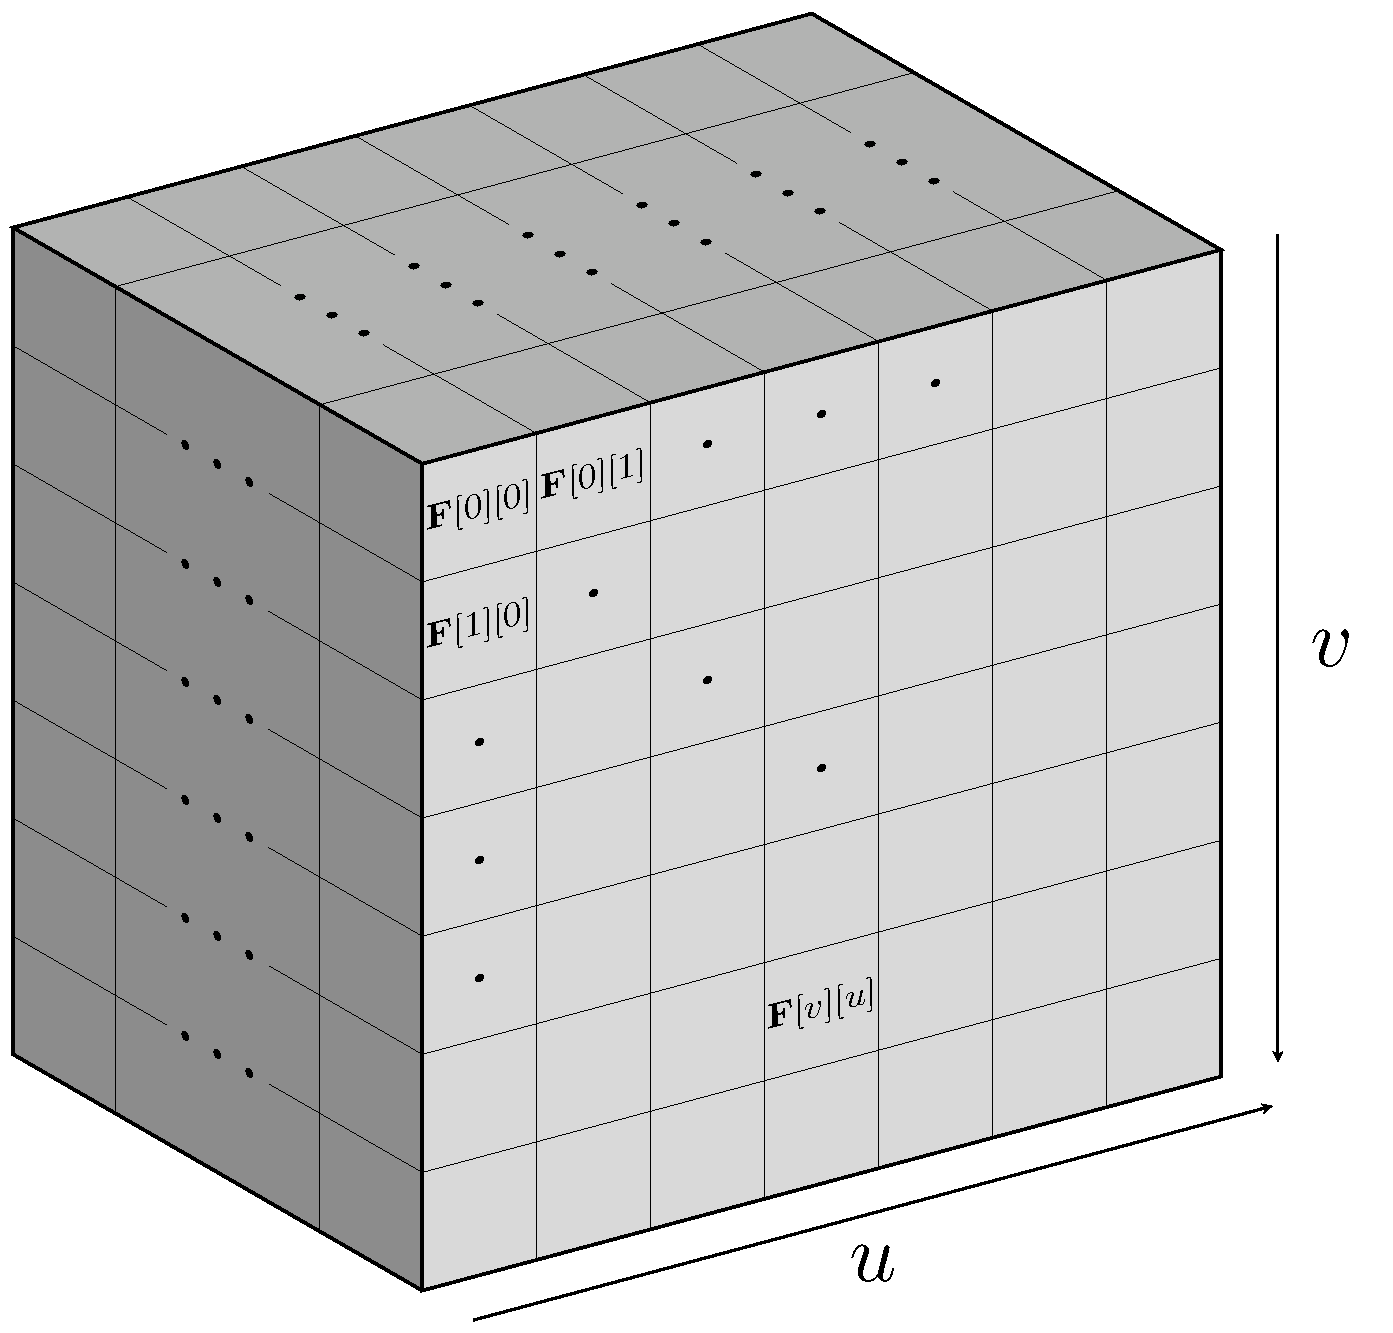
\includegraphics[width=\linewidth]{weights_input_dataset}
        \caption{A Tensor representing the Input Dataset $\tens{F}$}
        \label{fig:A Tensor representing the complete Input Dataset}
    \end{subfigure}
    \begin{subfigure}{.35\textwidth}
        \centering
        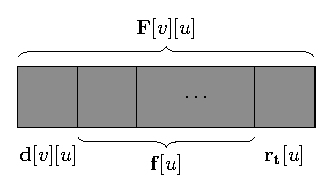
\includegraphics[width=\linewidth]{zoomup_Fuv}
        \caption{Contents of $\tens{F}[v][u]$: This vector (length $n_F$) contains quantified causes for the change in agents' behavior from $\matr{x_t}$ to $\matr{y_t}$}
        \label{fig:Zoomed-in contents of Fvu}
    \end{subfigure}
    \caption{Visual representation of the Input Dataset}
    \label{fig:Visual representation of the Input Dataset}
\end{figure}
Since preprocessing the dataset reduces data operations during model execution, the input dataset, comprising of distance between locations $\matr{D}$, environmental features $\vect{f}$ and given rewards $\vect{r_t}$ (all normalized), is built into a tensor (\Cref{fig:A Tensor representing the complete Input Dataset}) such that operations can be performed on batches of slices $\tens{F}[v]$.

Another advantage of building the dataset as a tensor comes with the Pytorch library, which provides convenient handling and transfer of tensors residing on the Main Memory and GPUs' internal global memory \cite{PTDocs}. \Cref{alg:Constructing the Input Dataset} describes the steps to construct this dataset.
\begin{algorithm}
    \caption{Constructing the Input Dataset} \label{alg:Constructing the Input Dataset}
    \begin{algorithmic}[1]
        \Function{Build-Dataset}{$\matr{D}, \matr{f}, \matr{r_t}$}
        \State $\matr{D} \gets \Call{Normalize}{\matr{D}}$\Comment{$\matr{D}[u][v]$ is the distance between locations $u$ and $v$}
        \State $\vect{f} \gets \Call{Normalize}{\mathbf{f}, axis = 0}$\Comment{$\mathbf{f}[u]$ is a vector of env. features at location $u$}
        \State $\vect{r_t} \gets \Call{Normalize}{\vect{r_t}, axis = 0}$\Comment{$\vect{r_t}[u]$ is the reward at location $u$}
        \For{$v = 1, 2, \dots, J$}
            \For{$u = 1, 2, \dots, J$}
                \State $\tens{F}[v][u] \gets [\matr{D}[v][u], \vect{f}[u], \vect{r_t}[u]]$ \Comment{As depicted in \Cref{fig:Zoomed-in contents of Fvu}}
             \EndFor
        \EndFor
        \State \Return $\matr{F}$
        \EndFunction
    \end{algorithmic}
\end{algorithm}

\subsection{Minimizing Loss for the Identification Problem} \label{sec:Minimizing Loss for the Identification Problem}
As shown in \Cref{fig:Neural network designed for the Identification Problem}, the neural network is made of 3 fully connected layers - the input layer, the hidden layer with rectified Linear Units (reLU), and the output layer with softmax$(\cdot)$ function units. The network can also be visualized as a stack of 1-dimensional layers (\Cref{fig:Side view of the network}), with the softmax$(\cdot)$ calculated on the stack's output.
\begin{figure}[!htbp]
    \centering
    \begin{subfigure}{\textwidth}
        \centering
        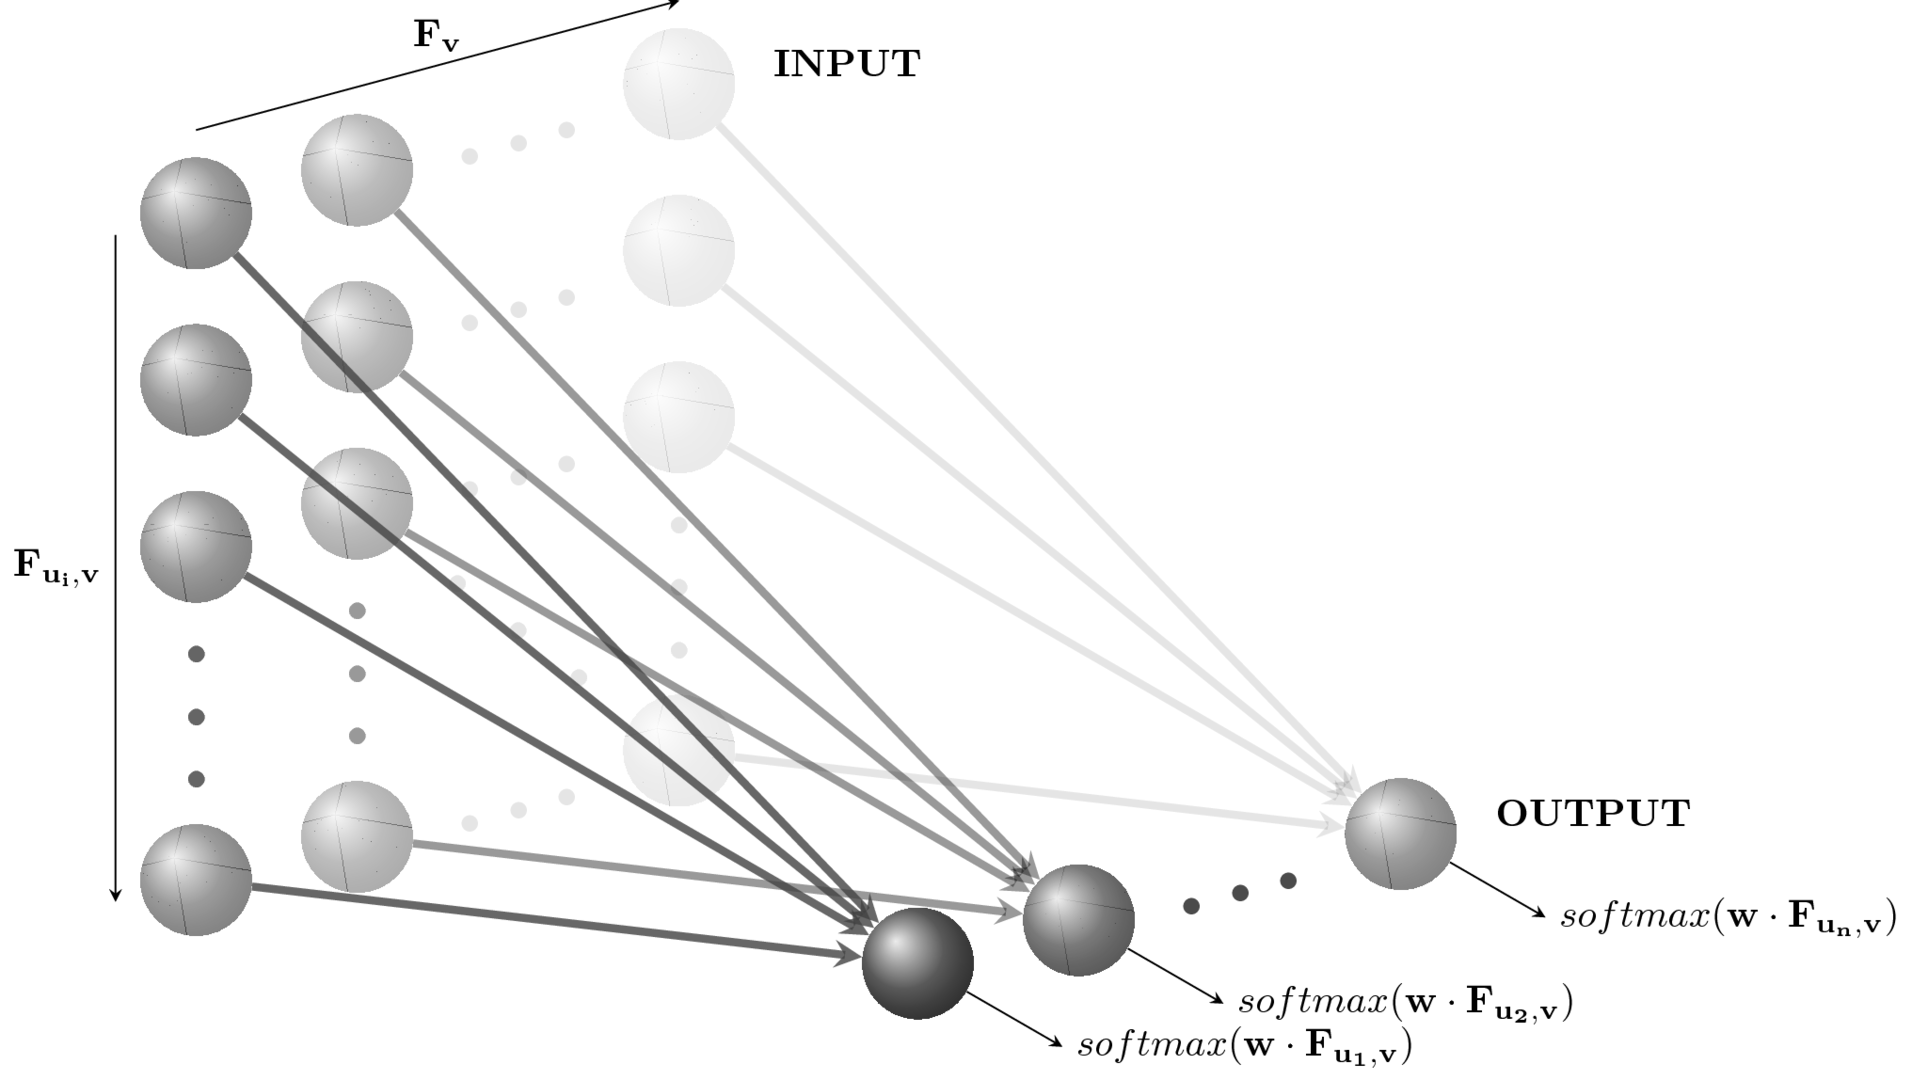
\includegraphics[width=\textwidth]{weights_net}
        \caption{3-dimensional View of the Network Slice, Taking in $\matr{F}[v]$}
        \label{fig:3-dimensional view of the network slice taking in Fv}
    \end{subfigure}
    \begin{subfigure}{.75\textwidth}
        \centering
        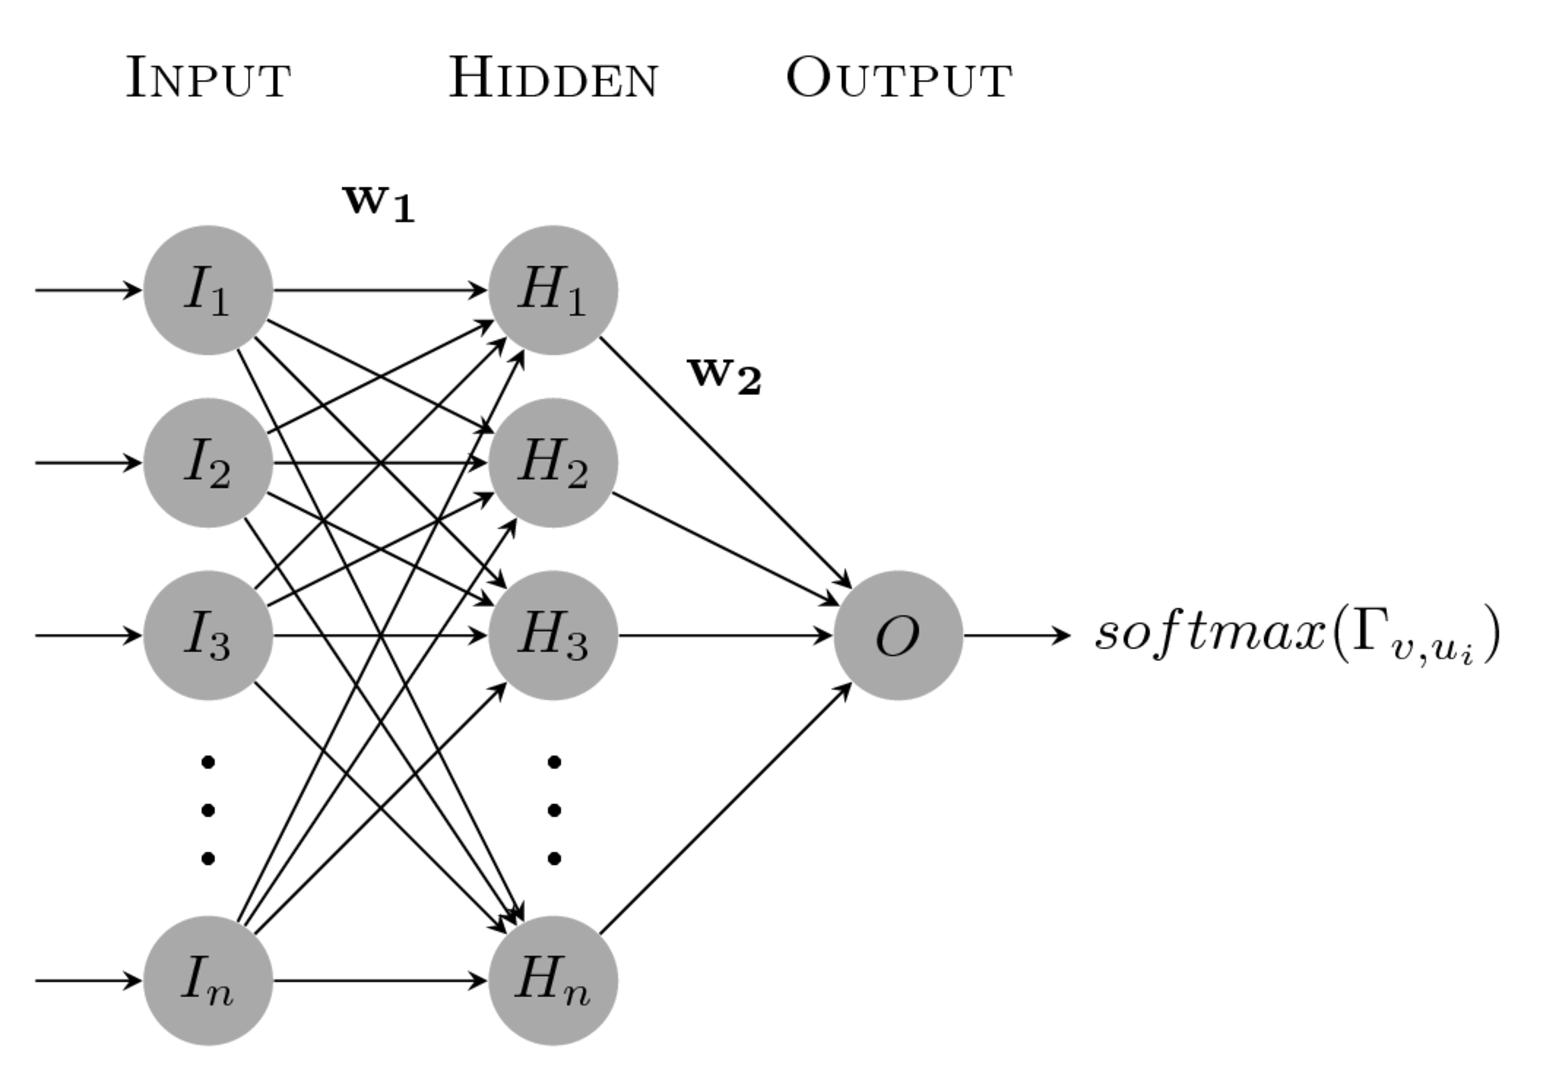
\includegraphics[width=\textwidth]{weights_net_side}
        \caption{Side View of the Network: Output of one such cross-section is $p_{u_i, v}$}
        \label{fig:Side view of the network}
    \end{subfigure}
    \caption{Neural Network Designed for the Identification Problem}
    \label{fig:Neural network designed for the Identification Problem}
\end{figure}

It is important to clarify that the network in \Cref{fig:3-dimensional view of the network slice taking in Fv}, which takes in $\matr{F}[v]$ as shown, is a slice of the original network, which takes in the complete tensor $\matr{F}$ and computes the complete result $\matr{P}^{T}$  per iteration of $t$. In other words, the input and the hidden layers are 3-dimensional, and the output layer is 2-dimensional. Since it is difficult to visualize the complete network on paper, slices of the network are depicted in \Cref{fig:3-dimensional view of the network slice taking in Fv}. \Cref{alg:Algorithm for the Identification Problem} details the steps for learning the parameters $\matr{w_1}$ and $\matr{w_2}$ based on \Cref{eqn:iden_problem,eqn:puv_equation}.

\begin{algorithm}
    \caption{Algorithm for the Identification Problem} \label{alg:Algorithm for the Identification Problem}
    \begin{algorithmic}[1]
        \State $\matr{w_1} \gets \Call{Random}{\;(J,n_F,n_F)\;}$\Comment{$\matr{w_1}$ has dimensions $J \times n_F \times n_F$}
        \State $\matr{w_2} \gets \Call{Random}{\;(J,n_F,1)\;}$\Comment{$\matr{w_2}$ has dimensions $J \times n_F \times 1$}
        \For{$e = 1, 2, \dots, \text{Epochs}$}
            \State $loss \gets 0$
            \For{$t = 1, 2, \dots, T$}
                \State $\matr{F} \gets \Call{Build-Dataset}{\matr{D}, \matr{f}, \matr{r}[t]}$\Comment{Defined in Algorithm \Cref{alg:Constructing the Input Dataset}}
                \State $\matr{H} \gets  \text{reLU}(\Call{Batch-Multiply}{\matr{F}, \matr{w_1}})$
                \State $\matr{O} \gets \text{softmax}(\Call{Batch-Multiply}{\matr{H}, \matr{w_2}})$
                \State $\matr{P} \gets \matr{O}^T$
                \State $loss \gets loss + (\omega(\matr{y}[t] - \matr{P} \cdot \matr{x}[t]))^2$
            \EndFor
            \State $\Call{Gradient-Descent}{loss, \matr{w_1}, \matr{w_2}}$
            \State $\matr{w_1}, \matr{w_2} \gets \Call{Update-Using-Gradients}{\matr{w_1}, \matr{w_2}}$
            \State $\Call{Log-Info}{e, loss}$
        \EndFor
    \end{algorithmic}
\end{algorithm}

\section{Pricing Problem} \label{sec:Pricing Problem}
After learning the set of weights $\matr{w_1}$ and $\matr{w_2}$ highlighting the change in agents' behavior to collect observations, the Pricing Problem aims to redistribute rewards to the all locations such that the predicted behavior of agents influenced by the new set of rewards is homogeneous. Thus, given a budget of rewards $\mathcal{R}$, this optimization problem can be expressed as:
\begin{equation} \label{eqn:pricing_problem}
    \begin{aligned}
        & \underset{\vect{r}}{\text{minimize}}
        & & Z_P(\vect{r}) = \frac{1}{n}\lVert \vect{y} - \mean{\vect{y}} \rVert\\
        & \text{subject to}
        & & \vect{y} = \matr{P}(\matr{f}, \vect{r}; \matr{w_1}, \matr{w_2}) \, \vect{x}\\
        &&& \sum_{i} r_i \leq \mathcal{R}\\
        &&& r_i \geq 0
    \end{aligned}
\end{equation}
where elements of $\matr{P}$ are defined as in \Cref{eqn:puv_equation}.

To allocate the rewards $\vect{r}$ optimally, the calculations for the pricing problem are akin to that for the Identification Problem (see \Cref{sec:Identification Problem}). However, since only 1 set of rewards need to be optimized, we use an altered 2-layer (input and output layers) network instead of the 3-layered network used for the Identification Problem. While \Cref{eqn:pricing_problem} looks like a typical Linear Programming problem, only a part of the formulation uses LP to constrain the rewards. We calculate $\matr{P}$ using a 2-layered network that minimizes the loss function $Z_P(\vect{r})$ using gradient descent, and constrain the rewards using linear programming. Fundamental processes are described below, whereas specific implementation details, with code optimizations and more data preprocessing, are described in \Cref{app:Implementation}.

\subsection{Input Dataset for Finding Rewards}
Since it is the set of rewards $\vect{r}$ that need to be optimized, they must serve as the ``weights'' of the network (``weights'' here refer to the weighted edges of this network and not to the set of calculated weights $\matr{w_1}$ and $\matr{w_2}$). Therefore, the rewards $\vect{r}$ are no longer fed into the network but are its characteristic. Instead, the calculated weights $\matr{w_1}$ are fed into the network, and are ``weighted'' by the rewards.

The observation density datasets, $\matr{x}$ and $\matr{y}$, are also aggregated for all agents such that they give information in terms of locations $u$ only. This is also why rewards vector $\vect{r}$ does not depend on $t$ - we want a generalized set of rewards for all time $t$ per location $u$. Therefore, the algorithm for constructing $\matr{F}$ (see \Cref{sec:Structure of Input Dataset for Identifying Weights}) is same as \Cref{alg:Constructing the Input Dataset} but with a change - $\vect{r_t}$ replaced by $\vect{r}$.

\subsection{Calculating Rewards} \label{sec:Calculating Rewards}
\Cref{alg:Solving the Pricing Problem} for finding $\matr{P}$ is very similar to \Cref{alg:Algorithm for the Identification Problem}'s first few steps but without any epochs of $t$. Also, since the model would predict $\vect{y}$, it does not need labels $\vect{y}$ as a dataset. Although \Cref{alg:Solving the Pricing Problem}'s logic flow may seem arcane, it is straight-forward - as displayed in \Cref{fig:Logic Flow of Algorithm Pricing Problem}.
\begin{figure}[!htbp]
    \centering
    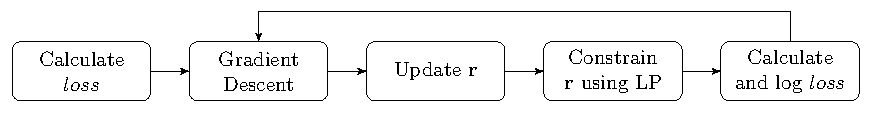
\includegraphics[width=\textwidth]{logic_alg_pricing}
    \caption{Logic Flow of \Cref{alg:Solving the Pricing Problem}}
    \label{fig:Logic Flow of Algorithm Pricing Problem}
\end{figure}
\begin{algorithm}
    \caption{Solving the Pricing Problem} \label{alg:Solving the Pricing Problem}
    \begin{algorithmic}[1]
        \Function{Forward}{$\matr{D}, \matr{f}, \vect{r}, \matr{w_1}, \matr{w_2}, \vect{x}$}
            \State $\matr{F} \gets \Call{Build-Dataset}{\matr{D}, \matr{f}, \vect{r}}$\Comment{Defined in  \Cref{alg:Constructing the Input Dataset}}
            \State $\matr{O}_1 \gets \text{reLU}(\Call{Batch-Multiply}{\matr{F}, \matr{w_1}})$
            \State $\matr{O}_2 \gets \text{softmax}(\Call{Batch-Multiply}{\matr{O}_1, \matr{w_2}})$
            \State $\matr{P} \gets \matr{O}_2^T$
            \State $\vect{y} \gets \matr{P} \cdot \vect{x}$
            \State \Return $\lVert \vect{y} - \mean{\vect{y}} \rVert / J$
        \EndFunction
        \vspace*{-.7\baselineskip}\Statex\hspace*{\dimexpr-\algorithmicindent-2pt\relax}\rule{\textwidth}{0.1pt}%
        \Statex\hspace*{-\algorithmicindent}\textbf{Main Script}%
        \vspace*{-.6\baselineskip}\Statex\hspace*{\dimexpr-\algorithmicindent-2pt\relax}\rule{\textwidth}{0.1pt}% horizontal rule
        \State $\vect{r} \gets \Call{Random}{\;(J)\;}$\Comment{$\vect{r}$ has dimensions $J$}
        \State $loss \gets \Call{Forward}{\matr{D}, \matr{f}, \vect{r}, \matr{w_1}, \matr{w_2}, \vect{x}}$
        \For{$e = 1, 2, \dots, \text{Epochs}$}
            
        \State $\Call{Gradient-Descent}{loss, \vect{r}}$
        \State $\vect{r} \gets \Call{Update-Using-Gradients}{\vect{r}}$
        \State $\vect{r} \gets \Call{LP}{\vect{r}, \mathcal{R}}$\Comment{LP($\cdot$) explained in \Cref{sec:Constraining Rewards}}
        \State $loss \gets \Call{Forward}{\matr{D}, \matr{f}, \vect{r}, \matr{w_1}, \matr{w_2}, \vect{x}}$
        \State $\Call{Log-Best-Rewards}{loss, \vect{r}}$\Comment{Record $\vect{r}$ with the lowest $loss$ yet}
        \EndFor
    \end{algorithmic}
\end{algorithm}

\subsection{Constraining Rewards} \label{sec:Constraining Rewards}
After updating the rewards, the program constrains them using LP($\cdot$) such that $\sum_{i}r_i \leq \mathcal{R}$ and $r_i \geq 0$. To do so, the LP($\cdot$) finds another set of rewards $\vect{r'}$ such that the absolute difference between new and old rewards ($\sum_{i}|r'_i - r_i|$) is minimum. The mathematical formulation is given in \Cref{eqn:lp_math_constrain_rewards}, which was implemented using SciPy's Optimize Module \cite{SCPOptimizeDocs}. Since the module supports a standard format for doing linear programming, \Cref{eqn:lp_code_constrain_rewards} is used (see \Cref{app:Implementation}), which is mathematically equivalent to \Cref{eqn:lp_math_constrain_rewards}.
\begin{multicols}{2}
    \begin{equation} \label{eqn:lp_math_constrain_rewards}
        \begin{aligned}\\
            & \underset{\vect{r'}}{\text{minimize}}
            & & \sum_{i}|r'_i - r_i|\\
            & \text{subject to}
            & & \sum_{i}r'_i \leq \mathcal{R}\\
            &&& r_i \geq 0\\ \\
        \end{aligned}
    \end{equation}\break
    \begin{equation} \label{eqn:lp_code_constrain_rewards}
        \begin{aligned}
            & \underset{[\vect{r'}, \vect{u}]}{\text{minimize}}
            & & \sum_{i} u_i\\
            & \text{subject to}
            & & r'_i - r_i \leq u_i\\
            &&& r_i - r'_i \leq u_i\\
            &&& \sum_{i} r'_i \leq \mathcal{R}\\
            &&& r'_i, u_i \geq 0
        \end{aligned}
    \end{equation}
\end{multicols}

We make a tradeoff by constraining rewards using LP instead of Mixed Integer Programming, which the previous study used \cite{Xue2016Avi2}. The tradeoff exists between decreasing the computation time and loosening integer constraints on each reward value. While model-learned integer rewards have worked in real-life testing also \cite{Xue2016Avi2}, we cannot say if allowing non-integer values in rewards would produce better results in real-life, corresponding to the model's prediction. In other words, we can't ensure the predicted rewards' effectiveness in ground testing before \textit{actually} deploying them in the game. Nevertheless, we can estimate how good the predictions can be compared to several baseline indicators. These baseline sets are elaborated in \Cref{sec:Pricing Problem-Optimizing the Original Dataset}.
    \chapter{Experiment Specifications} \label{sec:Experiment Specifications}
\begin{mydef} \label{def:GPU Speedup}
    GPU Speedup: Ratio of model's execution time with GPU ``set'' to that with CPU ``set''. The script's data preprocessing runtime is ignored, but the time taken to transfer data from CPU to GPU is included in calculating GPU ``set'' time elapsed. (Speedup = $\frac{CPU-time}{GPU-time\; +\; Transfer-time}$)
\end{mydef}

To test both our models, we conducted several tests for optimization and GPU Speedup. After initializing all parameters randomly (with specific seeds for reproduction and uniformity between tests), the models were run for 1000 or 10000 epochs depending on the complexity of the model.

\section{Datasets} \label{sec:Datasets}
We conducted two types of tests: \textbf{optimization tests on original datasets} and \textbf{GPU Speedup tests on randomly generated datasets}. Data was loaded or generated as Floating Point 32 (FP32) units, but was stored with less precision (up to 15 significant figures) to reduce secondary memory usage.

For the GPU Speedup runs, two random datasets of 173 time units ($T$) were generated beforehand using NumPy (without any seed):
\begin{enumerate} 
    \item 116 locations - for Identification Problem
    \item 232 locations - for Pricing Problem
\end{enumerate}

We used more locations for the Pricing Problem's model because its 2-layered network was less complex and time consuming than the Identification Problem's 3-layered network. Additionally, we took this step after initially testing the Pricing Problem on 116 locations but failing to obtain a clear trend (more in \Cref{sec:PriProbRes - GPU}). We believe that speedup tests on original datasets would give similar results, though we used randomly generated datasets because it was easier to scale and build random datasets of different batch-sizes for testing. The models were timed for the executed operations in a neural network and the LP, including transfer times of tensors between the RAM and GPU's internal memory. Time taken for preprocessing was ignored. 

\section{Test-Machine Configuration} \label{sec:Test-Machine Configuration}
Hardware specifications and software versions used for the experiments are listed in \Cref{tab:Hardware Specifications and Software Versions Used for Experiments}. Though we couldn't eliminate extraneous computing usage by background processes on the test-machine, we restricted background processes by switching off X (Graphical User Interface for Ubuntu OS) and performing tests in CLI (Command Line Interface), and ending user processes. Background processes and threads might give varying runtimes when other experiments are performed. However, one should obtain similar GPU Speedup results when repeating the experiments.
\begin{table}[!htbp]
    \centering
    \caption{Hardware Specifications and Software Versions Used for Experiments}
    \label{tab:Hardware Specifications and Software Versions Used for Experiments}
    \begin{tabular}{|c|c|}
        \hline
        \multicolumn{2}{c}{\textbf{Hardware}}\\
        \hline
        \textbf{Type} & \textbf{Unit/Specs}\\
        \hline
        Desktop & Dell Precision Tower 3620\\
        CPU & Intel Core i7-7700K\tablefootnote{Hyper-threaded with 4 cores, 8 threads @ 4.20-4.50 GHz}\\
        RAM & 16GB\\
        GPU & NVIDIA Quadro P4000\tablefootnote{1792 CUDA Cores @ 1.2-1.5 GHz}\\
        \hline
    \end{tabular}\quad
    \begin{tabular}{|c|c|}
        \hline
        \multicolumn{2}{c}{\textbf{Software}}\\
        \hline
        \textbf{Library/Package} & \textbf{Version}\\
        \hline
        Ubuntu OS & 16.04.2 LTS x86\textunderscore64\\
        CUDA & 8.0\\
        cuDNN & 5.1.10\\
        MKL & 2017.0.3\\
        Python & 2.7.13 (Anaconda)\\
        PyTorch & 0.1.12\textunderscore2\\
        NumPy & 1.12.1\\
        SciPy & 0.19.0\\
        \hline
    \end{tabular}
\end{table}

\paragraph{GPU ``set'' and CPU ``set'' Clarification}
By GPU ``set'' we mean \textit{distributing} operations in the scripts between CPU and GPU, while by CPU ``set'' we mean that the operations were executed \textit{only} on the CPU. Since GPUs are inferior than CPUs at handling most operations other than simple arithmetic matrix ones due to parallelism (see \Cref{sec:Computation Using GPUs}), we used - and recommend using - both the CPU and the GPU in GPU ``set'' to handle operations each is superior at. However, since the models in \Cref{alg:Algorithm for the Identification Problem,alg:Solving the Pricing Problem} (not the full scripts) are primarily arithmetic operations on  tensors, it is clear that they were executed on the GPU when it was ``set'' and on the CPU when the CPU was ``set''. Other than this optimization, we did not specifically design any parallelized algorithm for either configurations, relying on the PyTorch's and NumPy-SciPy's inbuilt implementation.

\section{Algorithm Choice} \label{sec:Algorithm Choice}
On the algorithm side, we used Adam's algorithm for \textsc{Gradient-Descent}($\cdot$), after testing performances of several algorithms\footnote{PyTorch lets you choose the corresponding function/module} including but not limited to Stochastic Gradient Descent (SGD) \cite{SGD}, Adam's Algorithm \cite{Adam} and Adagrad \cite{Adagrad}. In \Cref{sec:Results}, we only discuss and show tests using the Adam's algorithm, since it was found to work best with both models over all test runs.

\section{Running the Identification Problem's Model} \label{sec:Running the Identification Problem's Model}
\subsection{Optimizing the Original Dataset} \label{sec:Identification Problem-Optimizing the Original Dataset}
The 3-layered neural network was run for 10000 epochs on the original dataset, which was split 80:20 for training and testing sets, with different learning rates = $\{10^{-2}, 10^{-3}, 10^{-4}, 10^{-5}\}$. Since we were aiming for optimization, we ran multiple tests (5 different seeds with each learning rate) of the model only with the GPU ``set''.

To compare this model's optimization results with other model structures, the previously studied 2-layered network \cite{Xue2016Avi2} and a 4-layered neural network were used. The 4-layered network had another hidden layer with reLU, equivalent to the hidden layer in the current 3-layered network in \Cref{fig:3-dimensional view of the network slice taking in Fv}. The results from the 2-layered network were obtained from the previous study, and those from the 4-layered network were attained on the same original dataset with same parameter values (learning rates, epochs etc.).

\subsection{Testing GPU Speedup on the Random Dataset} \label{sec:Identification Problem-Testing GPU Speedup on the Random Dataset}
After generating a random dataset and splitting it 80:20 for training and testing to predict performance on the original dataset, we ran our 3-layered model with different batch-sizes $T = 17, 51, 85, 129, 173$ ($J = 116$) and different seeds with both GPU and CPU ``set'', logging the elapsed time for model execution. The total time elapsed was averaged for a batch-size on a device, which were used to generate scatter/line plots (see \Cref{sec:IdProbRes - GPU}).

\section{Running the Pricing Problem's Model} \label{sec:Running the Pricing Problem's Model}
\subsection{Optimizing the Original Dataset} \label{sec:Pricing Problem-Optimizing the Original Dataset}
After obtaining the set of weights $\matr{w_1}$ and $\matr{w_2}$ optimized using different seeds, we tested to find the best rewards (with the lowest loss - \Cref{eqn:pricing_problem}) with random $\vect{r}$ initiation. To obtain the best rewards, the model was run on all sets of weights obtained from the Identification Problem for 1000 epochs with different learning rates. In search for the best rewards with the minimum loss, we took this approach:
\begin{enumerate}
    \item Run differently seeded rewards on all sets of weights obtained from the Identification Problem, and identify a set of weights which performed better than the others (low $Z_I$ - \Cref{eqn:pricing_problem}) on average. The learning rate was fixed to $10^{-3}$ in this case.
    \item Use that set of weights to run a number of tests with varying seeds and learning rates = $\{10^{-2}, 5 \times 10^{-3}, 10^{-3}, 5 \times 10^{-4}, 10^{-4}, 5 \times 10^{-5}, 10^{-5}\}$, and choose the rewards which gave the lowest loss value $Z_I$ anytime during execution\footnote{This means that we selected the rewards before completion if the loss at that epoch was lower than that in the end.}. 
\end{enumerate}

Two sets of rewards were tested for loss values as baseline comparisons to our model - a randomly generated set, and another with elements inversely proportional to the number of visits at each location. While the former was a random baseline, the latter captured the idea of allocating higher rewards to relatively under-sampled locations. The best loss values were compared for all tests with the baselines.

\subsection{Testing GPU Speedup on the Random Dataset} \label{sec:Pricing Problem-Testing GPU Speedup on the Random Dataset}
Initially, we ran the Pricing Problem's model with different batch-sizes $J = 11, 35, 55, 85, 116$ ($T = 173$) and different seeds with both GPU and CPU ``set''. Since we couldn't find a clear trend, we tested on more locations $J = 145, 174, 203, 232$.

We relied on SciPy's Optimize Module to solve our LP sub-problem (see \Cref{sec:Constraining Rewards}) because PyTorch does not provide a GPU-accelerated Simplex LP solver. Since SciPy's implementation does not utilize the GPU, we expected the LP problem to be executed on the CPU and thus deliver equal runtimes in both GPU and CPU ``set'' configurations.
    \chapter{Results} \label{sec:Results}
\section{Identification Problem's Results} \label{sec:Identification Problem's Results}
\subsection{Optimization Results} \label{sec:IdProbRes - Optimization}
Running the 3-layered network with the GPU ``set'' with different learning rates on different seeds (to calculate average performance of each learning rate) for 10000 epochs showed that the model was performing constantly giving lower loss values ($Z_I$ - \Cref{eqn:iden_problem}) with learning rate = $10^{-3}$. 

We observed that higher learning rates ($>10^{-2}$) could only decrease the loss function to a limit, after which the updates in the weights caused the loss function to oscillate and increase. This phenomena is exemplified in \Cref{fig:Test Loss Plots of Different Learning Rates to Find Weights}, which are plots of different models with the same seed but different learning rates. On the other side of $10^{-3}$, lower learning rates took too long to train. Runtime for the model on 10000 epochs was 1232.56 seconds (average over 20 runs = 5 seeds $\times$ 4 learning rates), and models with learning rates less than $10^{-3}$ did not perform better than those with learning rate = $10^{-3}$ on \textit{any} run. Although the decrease in test losses were constant for learning rates less than $10^{-3}$, we feel that they may be computationally expensive and temporally inconvenient to train.
\begin{table}[!htbp]
    \centering
    \caption[Loss Values Calculated for Different Models for Identification Problem]{Loss Values Calculated for Different Models for Identification Problem: For both the 3- and the 4-layered models, learning rate = $10^{-3}$ outperformed other learning rates. Consequently, that learning rate is used in comparison with other models in \Cref{fig:Comparison of Loss Values from Different Models of the Identification Problem}.}
    \label{tab:Loss Values Calculated for Different Models for Identification Problem}
    \begin{tabular}{c | c | c}
        \hline
        \multirow{2}{*}{\textbf{Learning Rate}} & \multicolumn{2}{c}{\textbf{Average Test Loss Values}} \\
        & 3-layered & 4-layered\\
        \hline
        $10^{-2}$ & 0.168 $\pm$ 0.068 & 0.494 $\pm$ 0.083\\
        $10^{-3}$ & \textbf{0.119 $\pm$ 0.016} & \textbf{0.228 $\pm$ 0.048}\\
        $10^{-4}$ & 0.151 $\pm$ 0.040 & 0.237 $\pm$ 0.067\\
        $10^{-5}$ & 0.212 $\pm$ 0.040 & 0.320 $\pm$ 0.067\\
        \hline
    \end{tabular}
\end{table}

\begin{figure}[!htbp]
    \centering
    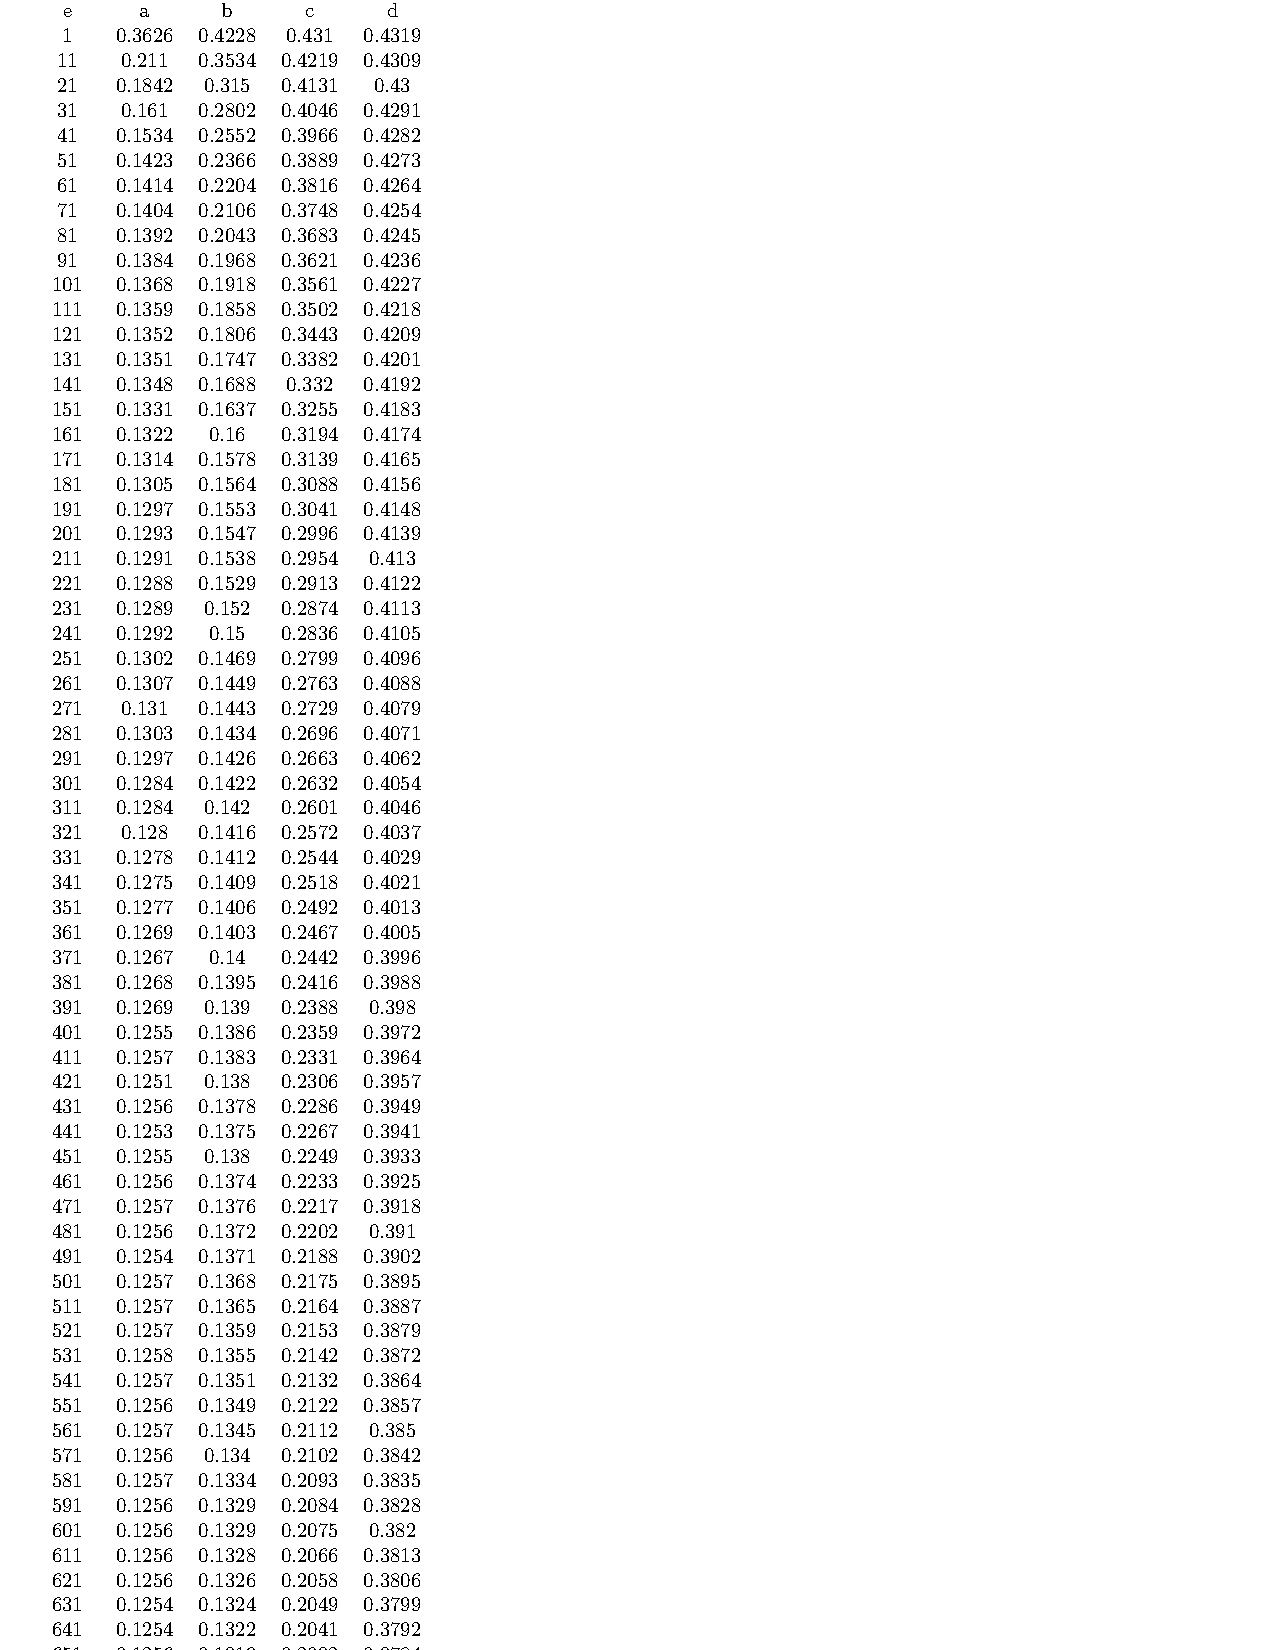
\includegraphics[width=16cm, height=10cm]{test_losses_diff_lr_plot}
    \caption{Test Loss Plots of Different Learning Rates to Find Weights}
    \label{fig:Test Loss Plots of Different Learning Rates to Find Weights}
\end{figure}
\begin{figure}[!htbp]
    \centering
    \begin{minipage}{.48\textwidth}
        \centering
        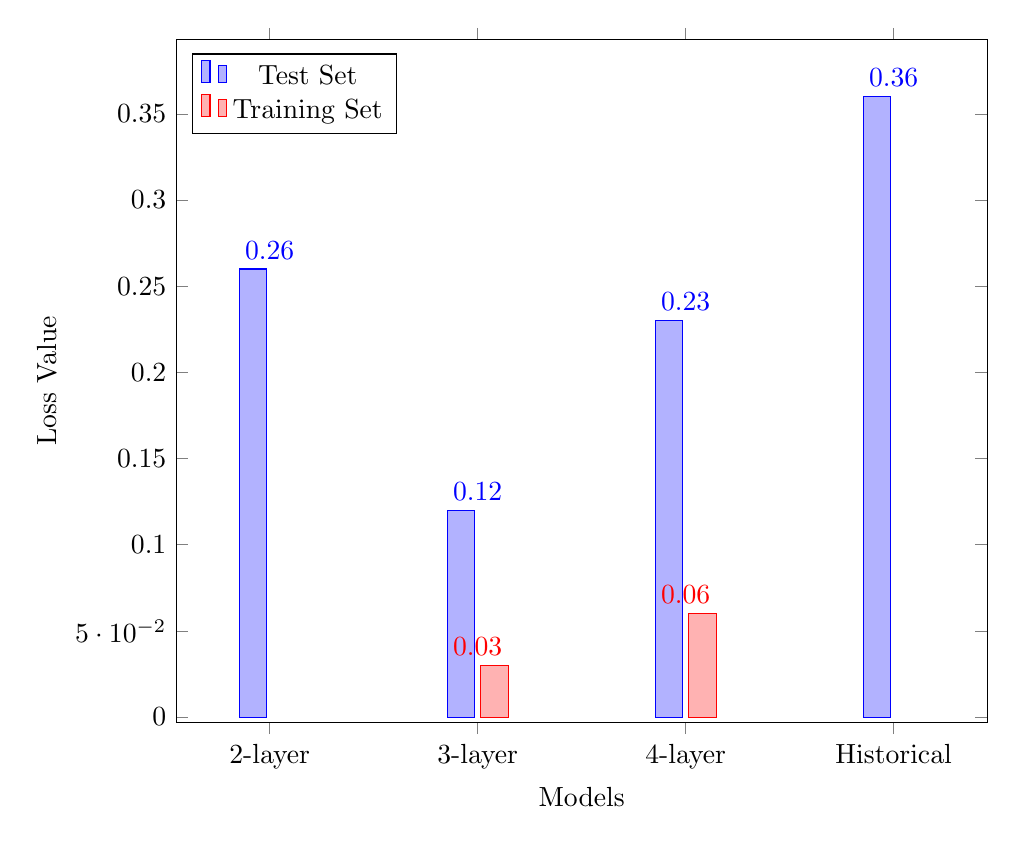
\begin{tikzpicture}
            \begin{axis}[
                ybar,
                width=.98\textwidth,
                enlarge x limits=0.15,
                legend style={at={(0.02,0.98)},
                    anchor=north west,legend columns=1},
                ylabel={Loss Value},
                symbolic x coords={2-layer,3-layer,4-layer, Historical},
                xtick=data,
                nodes near coords,
                nodes near coords align={vertical},
                every node near coord/.style={/pgf/number format/fixed},
                xlabel={Models},
            ]
            \addplot coordinates {(2-layer,0.26) (3-layer,0.12) (4-layer,0.23) (Historical, 0.36)};% test set
            \addplot coordinates {(3-layer,0.03) (4-layer,0.06)};% training set
            \legend{Test Set,Training Set}
            \end{axis}
        \end{tikzpicture}
        \caption[Comparison of Loss Values from Different Models of the Identification Problem]{Comparison of Loss Values from Different Models of the Identification Problem: Loss values for the training set are inevitably lower than that for the test set, which should be the basis for comparison}
        \label{fig:Comparison of Loss Values from Different Models of the Identification Problem}
    \end{minipage}\hfill
    \begin{minipage}{.48\textwidth}
        \centering
        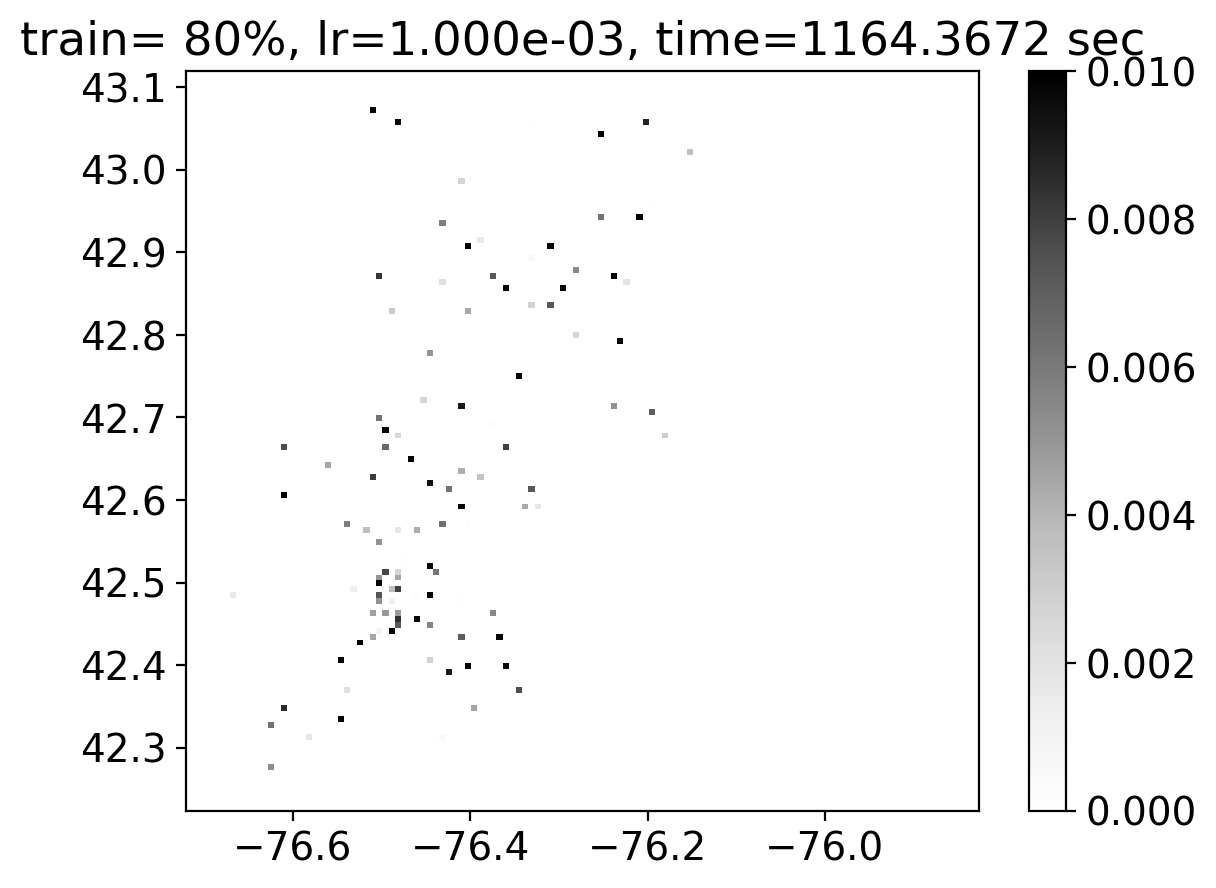
\includegraphics[width=\textwidth]{weights_map_plot_3}
        \caption[Predicted Probabilities of Agents Visiting Each Location Plotted on a Map (Latitude, Longitude) Representing Tompkins and Cortland Counties, NY]{Predicted Probabilities of Agents Visiting Each Location Plotted on a Map (Latitude, Longitude) Representing Tompkins and Cortland Counties, NY: Dark dots represent high prediction of visits. This can be compared to the plots for the 2-layered network and other models \cite[Figure 3]{Xue2016Avi2}.}
        \label{fig:Predicted Probabilities of Agents Visiting Each Location Plotted on a Map}
    \end{minipage}
\end{figure}

Observing that the average test loss values of learning rate = $10^{-3}$ is the lowest, we compare its results with the previous study's 2-layered network, historical data \cite[Table 1]{Xue2016Avi2}, and the 4-layered network with learning rate = $10^{-3}$ (see \Cref{sec:Identification Problem-Optimizing the Original Dataset}). As depicted in \Cref{fig:Comparison of Loss Values from Different Models of the Identification Problem}, our 3-layered neural network outperformed the previous 2-layered model by \textbf{0.14 units (14\% more closer to Ground Truth - $\matr{y}$)} \cite[Table 1]{Xue2016Avi2}, and also produced much better results (12\% more closer to Ground Truth) than the 4-layered model.

We also generated the predicted probabilities of the agents in the Test Set, visiting each location ($\matr{P}\matr{x}$), and plotted it onto maps marked by the locations' latitudes and longitudes. \Cref{fig:Predicted Probabilities of Agents Visiting Each Location Plotted on a Map} shows such a plot generated by the 3-layered network, where each dot represents a location.

To check if the model was overfitting at learning rate = $10^{-3}$, we plotted loss values at the end of each epoch for all tests. Although there remained $\approx$ 9\% difference (0.09 loss units) in the values of training and testing set, the 3-layered model was not drastically overfitting as an average \textit{end} difference of $8.76 \pm 1.59$\% persisted for many epochs, instead of increasing and tuning more to the training set. Even though one would expect overfitting with more tuned parameters, the 4-layered model also  produced an average \textit{end} difference of $16.77 \pm 4.73\%$, which persisted during the run. \Cref{fig:Train & Test Loss Values' Plots of Different Models} shows the results of a randomly selected experiment with plots of loss values at each epoch for the both networks.
\begin{figure}[!htbp]
    \centering
    \begin{subfigure}{.49\textwidth}
        \centering
        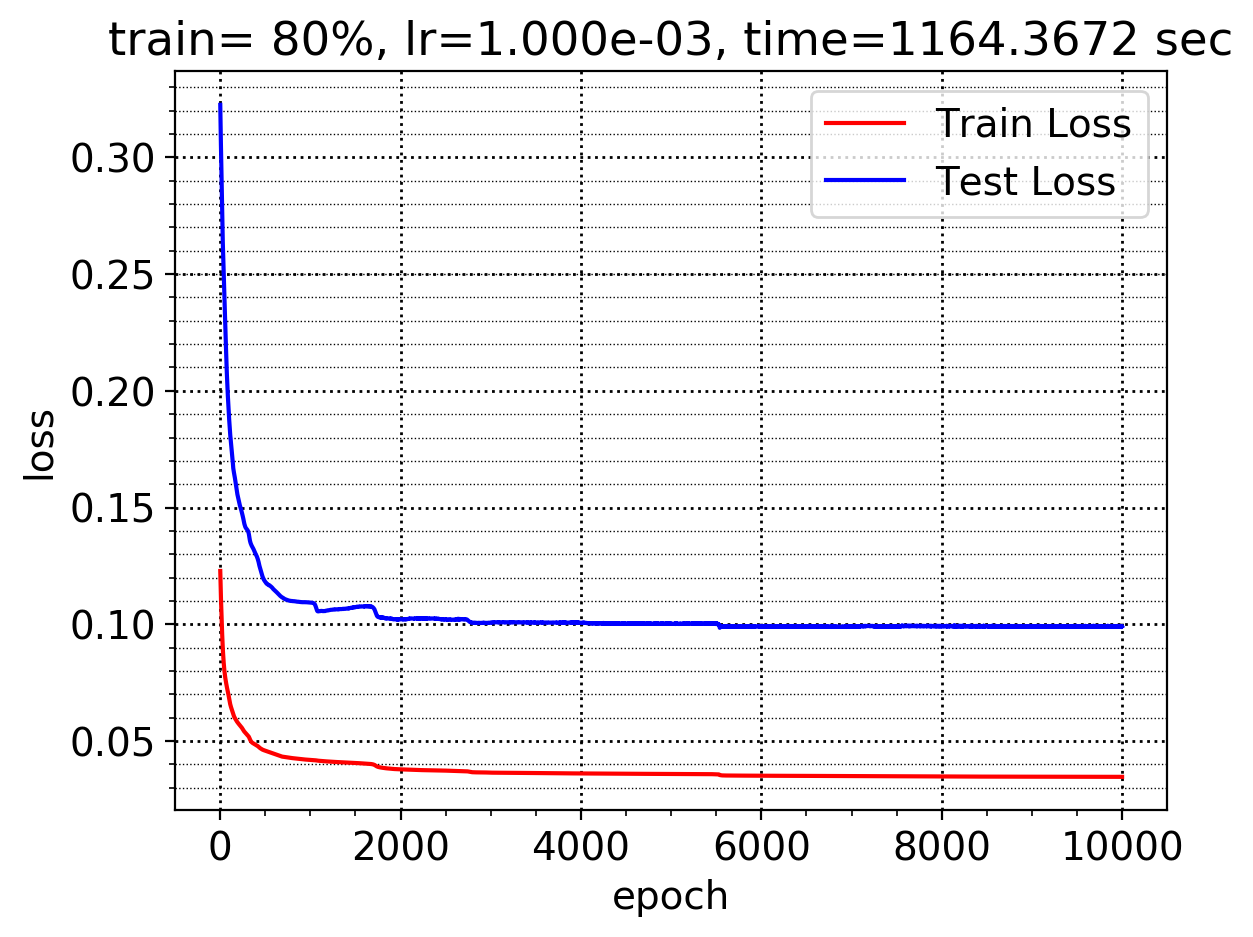
\includegraphics[width=\textwidth]{weights_train_test_loss_3_plot}
        \caption{Plot for 3-layered Model}
        \label{fig:Plot for 3-layered Model}
    \end{subfigure}
    \begin{subfigure}{.49\textwidth}
        \centering
        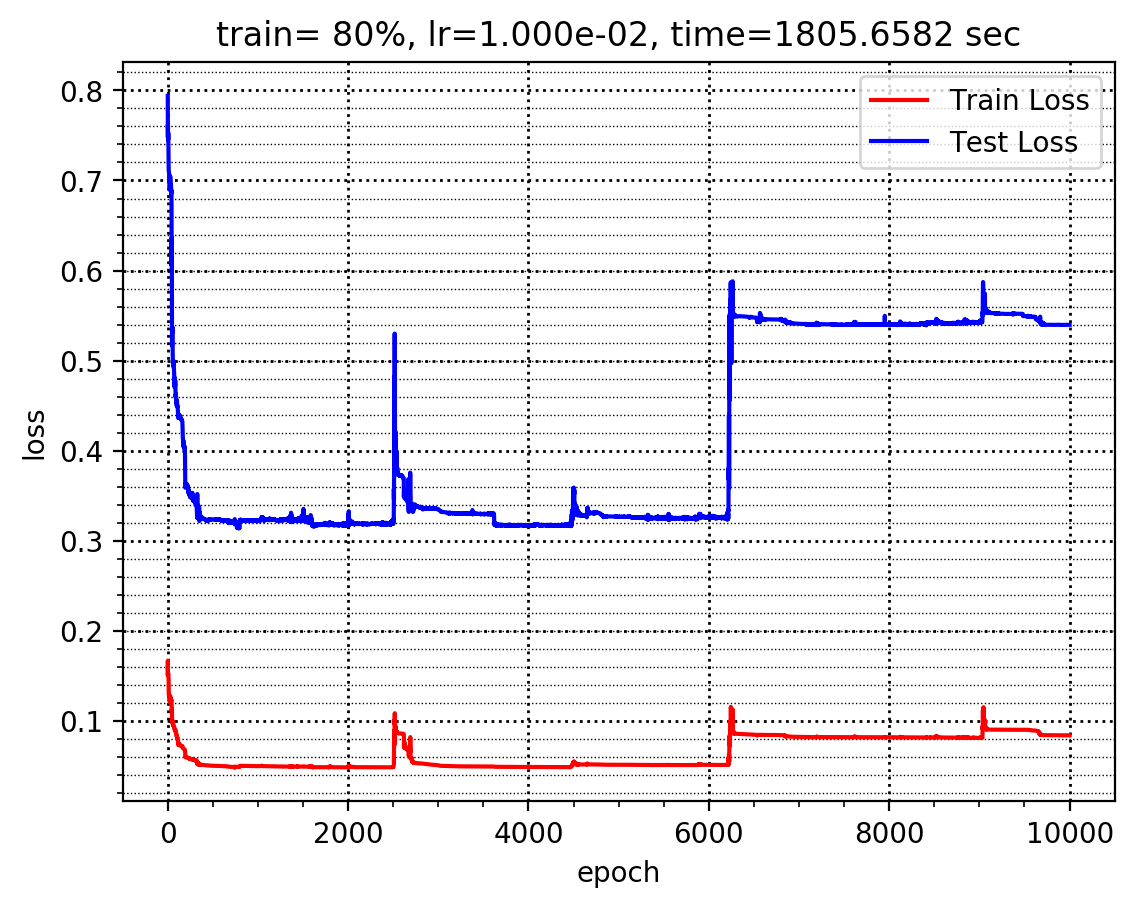
\includegraphics[width=\textwidth]{weights_train_test_loss_4_plot}
        \caption{Plot for 4-layered Model // todo}
        \label{fig:Plot for 4-layered Model}
    \end{subfigure}
    \caption[Train and Test Loss Values' Plots of Different Models]{Train and Test Loss Values' Plots of Different Models: Both networks learn the set of weights quickly, as displayed in the steep descent in loss values before $\approx$ 1000 epochs. This quick learning is due to the choice of \textsc{Gradient-Descent}($\cdot$) function - Adam's algorithm \cite{Adam}. Other algorithms like SGD \cite{SGD} and Adagrad \cite{Adagrad} learn relatively slowly.}
    \label{fig:Train & Test Loss Values' Plots of Different Models}
\end{figure}

\subsection{GPU Speedup Results} \label{sec:IdProbRes - GPU}
Running on batches of sizes $T = 17, 51, 85, 129, 173$ on a randomly generated dataset for 1000 epochs with both GPU and CPU ``set'' separately, we obtained information on full execution runtimes (both training and testing runtimes combined). The average results (over 3 different seeds for each batch) are plotted in \Cref{fig:Execution Times of Different Batch-Sizes with GPU and CPU ``set'' Separately}, which show promising GPU Speedup over CPU figures for any batch size; the GPU Speedup averaged over all tested batch-sizes is $\textbf{9.06}\pm\textbf{0.45}$.
\begin{figure}[!htbp]
    \centering
    \begin{subfigure}{.59\textwidth}
        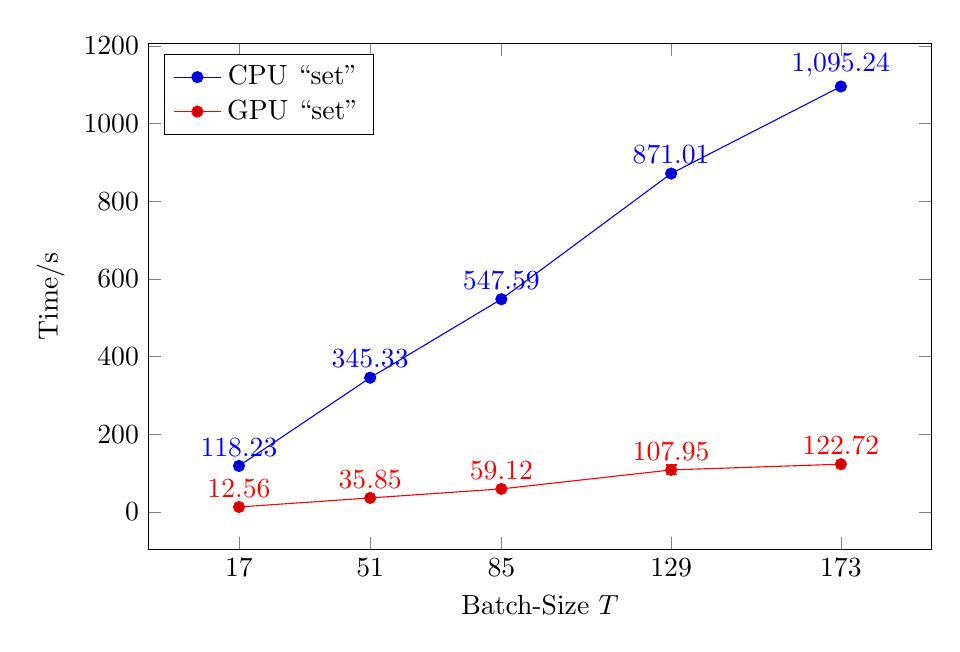
\begin{tikzpicture}
        \begin{axis}[
        width=.95\textwidth,
        height=8cm,
        xtick=data,
        xlabel={Batch-Size $T$},
        ylabel={Time/s},
        enlarge x limits=0.15,
        y tick label style={/pgf/number format/1000 sep=},
        extra y tick style={grid=major, tick label style={xshift=-1cm}},
        legend style={at={(0.02,.98)},
            anchor=north west},
        nodes near coords,
        ]
        \addplot+ [mark=*,error bars/.cd, y dir=both,y explicit] coordinates {
            (17,118.23) +- (1.77, 1.77)
            (51,345.33) +- (2.00, 2.00)
            (85,547.59) +- (1.76, 1.76)
            (129,871.01) +- (3.01, 3.01)
            (173,1095.24) +- (1.71, 1.71)
        };  % cpu
        \addplot+ [mark=*,error bars/.cd, y dir=both,y explicit] coordinates {
            (17,12.56) +- (0.022, 0.022)
            (51,35.85) +- (0.232, 0.232)
            (85,59.12) +- (0.131, 0.131)
            (129,107.95) +- (12.788, 12.788)
            (173,122.72) +- (0.169, 0.169)
        };  % gpu
        \legend{CPU ``set'',GPU ``set''}
        \end{axis}
        \end{tikzpicture}
    \end{subfigure}
    \begin{subfigure}{.4\textwidth}
        \centering
        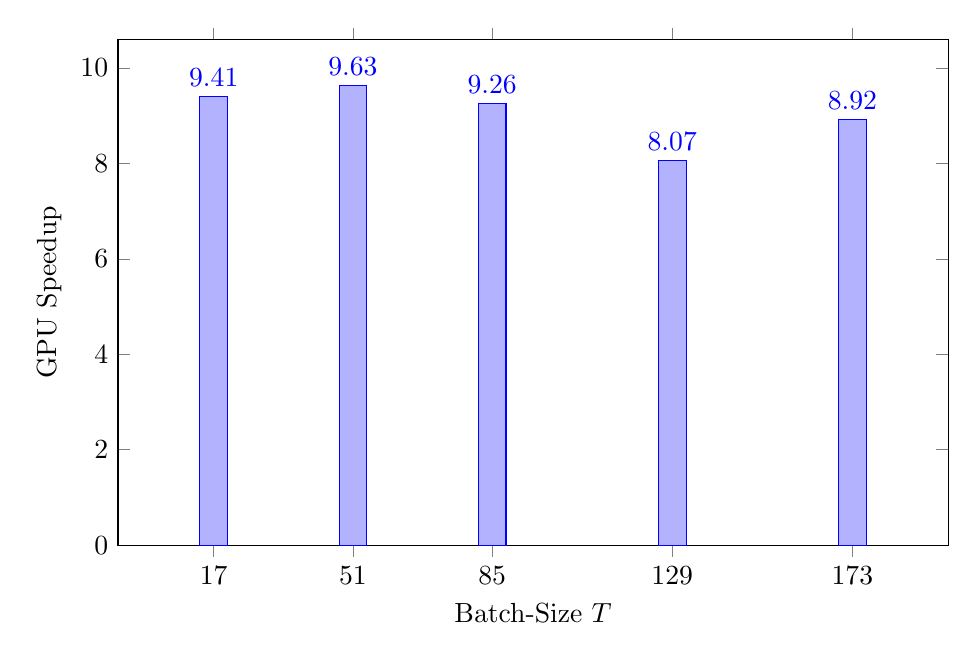
\begin{tikzpicture}
            \begin{axis}[
            ybar,
            width=\textwidth,
            height=8cm,
            xtick=data,
            xlabel={Batch-Size $T$},
            ylabel={GPU Speedup},
            ymin=0,
            enlarge x limits=0.15,
            extra y tick style={grid=major, tick label style={xshift=-1cm}},
            nodes near coords,
            ]
            \addplot+ coordinates {
                (17,9.41)
                (51,9.63)
                (85,9.26)
                (129,8.07)
                (173,8.92)
            };
            \legend{}
            \end{axis}
        \end{tikzpicture}
    \end{subfigure}
    \caption[Finding Weights - Execution Times of Different Batch-Sizes $T$ with GPU and CPU ``set'' Separately]{Finding Weights - Execution Times of Different Batch-Sizes $T$ with GPU and CPU ``set'' Separately: The GPU delivers faster computation than CPU even as the datasets' sizes grow - the average speedup is $9.06\pm0.45$. Also, the error bars are indiscernible because they are too small ($< 1\%$)}.
    \label{fig:Execution Times of Different Batch-Sizes with GPU and CPU ``set'' Separately}
\end{figure}

\section{Pricing Problem's Results} \label{sec:Pricing Problem's Results}
\subsection{Optimization Results} \label{sec:PriProbRes - Optimization}
Taking the approach mentioned in \Cref{sec:Pricing Problem-Optimizing the Original Dataset}, we obtained consistent loss values for each set of weights (even with differently seeded rewards). The best performing set of weights was set-2, using which the average loss value for the Pricing Problem hovered around $0.0079\%$. Next, running differently seeded rewards with different learning rates on set-2 of weights, we obtained the lowest loss value of $\textbf{0.0069\%}$.
%    \begin{figure}[!htbp]
%        \centering
%        \begin{tikzpicture}
%        \begin{axis}[
%        ybar,
%        width=.6\textwidth,
%        height=7cm,
%        enlarge x limits=0.15,
%        ylabel={Loss Value (in\%)},
%        symbolic x coords={Set-1,Set-2,Set-3,Set-4,Set-5},
%        xtick=data,
%        nodes near coords,
%        nodes near coords align={vertical},
%        xlabel={Models},
%        xlabel style={yshift=-.5cm}
%        ]
%        \addplot+ [error bars/.cd, y dir=both, y explicit] coordinates {
%            (Set-1, 0.0152) +- (0.0001, 0.0001)
%            (Set-2, 0.0079) +- (0.0005, 0.0005)
%            (Set-3, 0.0139) +- (0.0003, 0.0003)
%            (Set-4, 0.0129) +- (0.0002, 0.0002)
%            (Set-5, 0.0155) +- (0.0002, 0.0002)
%        };
%        \end{axis}
%        \end{tikzpicture}
%    \end{figure}

Compared to the proportional reward distribution (loss values calculated using set-2 of weights), our model's set of rewards produced loss value $\approx$ \textbf{3 times} lower. We again clarify that we compare the best loss values, as the organizer expects to find a distribution that is as optimal as possible.  \Cref{tab:Loss Values Calculated from Different Sets of Rewards} lists the best loss values obtained on each type of reward allocation (model's predicted, random and proportional - \Cref{sec:Pricing Problem-Optimizing the Original Dataset}).
\begin{table}[!htbp]
    \centering
    \caption[Loss Values Calculated from Different Sets of Rewards]{Loss Values Calculated from Different Sets of Rewards: The values are small because the loss function $Z_P(\vect{r})$ (\Cref{eqn:pricing_problem}) is averaged over the number of locations}
    \label{tab:Loss Values Calculated from Different Sets of Rewards}
    \begin{tabular}{|c|c|}
        \hline
        \textbf{Rewards Obtained From} & \textbf{Best Loss Values (In \%)}\\
        \hline
        Model's Prediction & 0.0069\\
        Random Initialization & 0.0331\\
        Proportional Distribution & 0.0235\\
        \hline
    \end{tabular}
\end{table}

\subsection{GPU Speedup Results} \label{sec:PriProbRes - GPU}
After running on different batch-sizes $J = 11, 35, 55, 85, 116, 145, 174, 203, 232$, we \textbf{did not observe drastic GPU speedup} for the full model. \Cref{fig:Finding Rewards - Time Taken by the Full Model} shows the Speedup trend: GPU Speedup for the full model was a mere \textbf{1.53 $\pm$ 0.10}.
\begin{figure}[!htbp]
    \centering
    \begin{subfigure}{\textwidth}
        \centering
        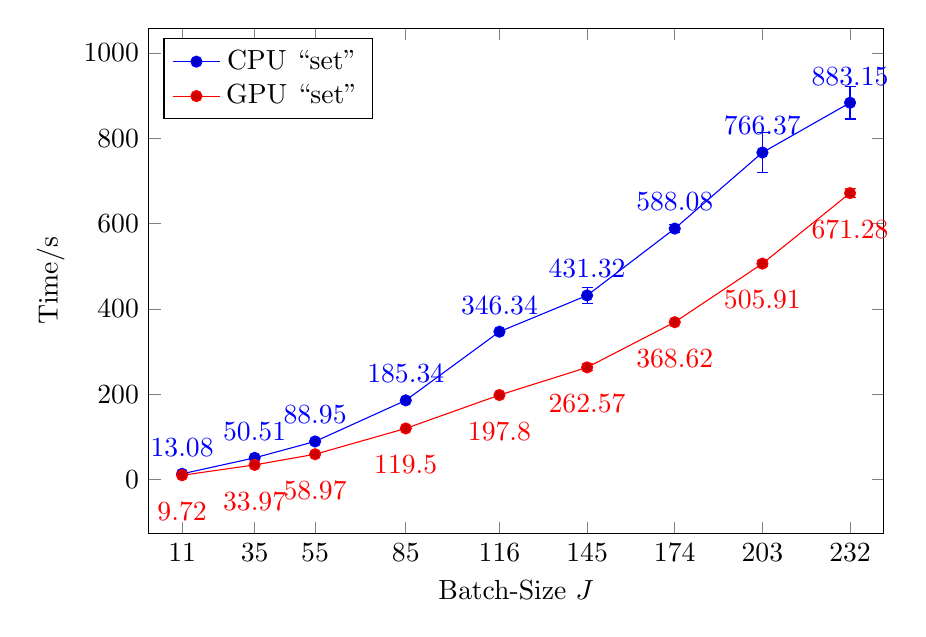
\begin{tikzpicture}
            \begin{axis}[
            width=.9\textwidth,
            height=8cm,
            xtick=data,
            xlabel={Batch-Size $J$},
            ylabel={Time/s},
            enlarge y limits=0.15,
            enlarge x limits=0.05,
            y tick label style={/pgf/number format/1000 sep=},
            extra y tick style={grid=major, tick label style={xshift=-1cm}},
            legend style={at={(0.02,.98)},
                anchor=north west},
            nodes near coords,
            every node near coord/.append style={yshift=-0.7cm}
            ]
            \addplot+ [mark=*,
            nodes near coords=\raisebox{0.8cm}{\pgfmathprintnumber\pgfplotspointmeta},error bars/.cd, y dir=both,y explicit
            ] coordinates {
                (11,13.08) +- (1.04, 1.04)
                (35,50.51) +- (1.73, 1.73)
                (55,88.95) +- (0.35, 0.35)
                (85,185.34) +- (0.95, 0.95)
                (116,346.34) +- (1.67, 1.67)
                (145,431.32) +- (18.06,18.06)
                (174,588.08) +- (10.16,10.16)
                (203,766.37) +- (47.02,47.02)
                (232,883.15) +- (38.00,38.00)
            };  % cpu
            \addplot+ [mark=*,error bars/.cd, y dir=both,y explicit] coordinates {
                (11,9.72) +- (0.08, 0.08)
                (35,33.97) +- (0.26, 0.26)
                (55,58.97) +- (0.19, 0.19)
                (85,119.50) +- (0.35, 0.35)
                (116,197.80) +- (4.02, 4.02)
                (145,262.57) +- (8.04,8.04)
                (174,368.62) +- (1.06,1.06)
                (203,505.91) +- (6.38,6.38)
                (232,671.28) +- (10.74,10.74)
            };  % gpu
            \legend{CPU ``set'',GPU ``set''}
            \end{axis}
        \end{tikzpicture}
        \caption{Time Taken by the Full Model: GPU Speedup over all batch-sizes is only \textbf{1.53 $\pm$ 0.10}.}
        \label{fig:Finding Rewards - Time Taken by the Full Model}
    \end{subfigure}\vspace*{1em}
    \begin{subfigure}{\textwidth}
        \centering
        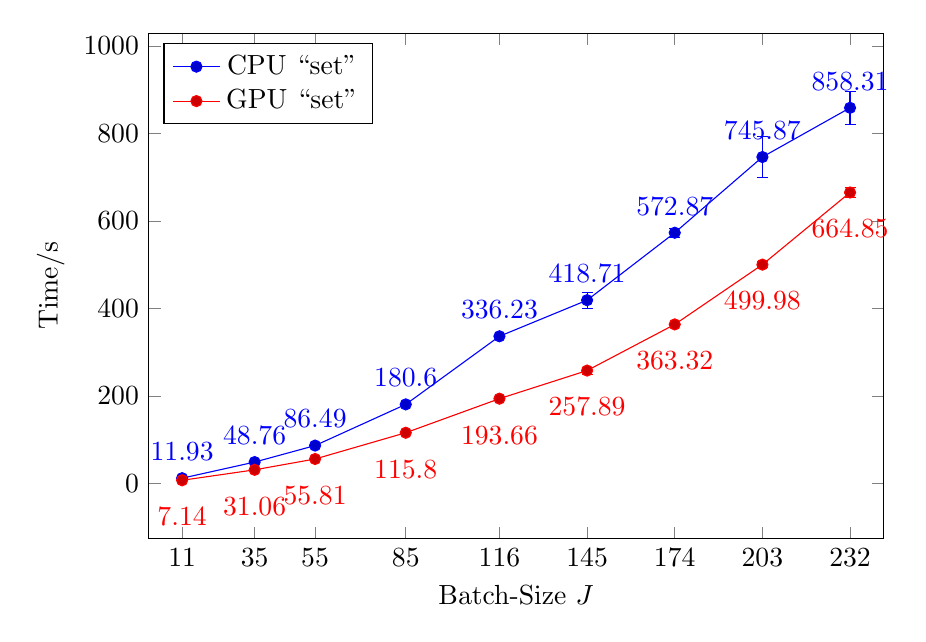
\begin{tikzpicture}
            \begin{axis}[
            width=.9\textwidth,
            height=8cm,
            xtick=data,
            enlarge y limits=0.15,
            enlarge x limits=0.05,
            xlabel={Batch-Size $J$},
            ylabel={Time/s},
            y tick label style={/pgf/number format/1000 sep=},
            legend style={at={(0.02,.98)},
                anchor=north west},
            nodes near coords,
            every node near coord/.append style={yshift=-0.7cm}
            ]
            \addplot+ [mark=*,
            nodes near coords=\raisebox{0.8cm}{\pgfmathprintnumber\pgfplotspointmeta},error bars/.cd, y dir=both,y explicit
            ] coordinates {
                (11,11.93) +- (0.94, 0.94)
                (35,48.76) +- (1.68, 1.68)
                (55,86.49) +- (0.36, 0.36)
                (85,180.60) +- (0.97, 0.97)
                (116,336.23) +- (1.46, 1.46)
                (145,418.71) +- (18.17,18.17)
                (174,572.87) +- (10.35,10.35)
                (203,745.87) +- (46.88,46.88)
                (232,858.31) +- (37.18,37.18)
            };  % cpu
            \addplot+ [mark=*,error bars/.cd, y dir=both,y explicit] coordinates {
                (11,7.14) +- (0.08, 0.08)
                (35,31.06) +- (0.26, 0.26)
                (55,55.81) +- (0.19, 0.19)
                (85,115.80) +- (0.35, 0.35)
                (116,193.66) +- (4.02, 4.02)
                (145,257.89) +- (8.01,8.01)
                (174,363.32) +- (1.03,1.03)
                (203,499.98) +- (6.37,6.37)
                (232,664.85) +- (10.73,10.73)
            };  % gpu
            \legend{CPU ``set'',GPU ``set''}
            \end{axis}
        \end{tikzpicture}
        \caption[Time taken by the LP]{Time taken by the LP: GPU Speedup over all batch-sizes is only \textbf{1.56 $\pm$ 0.08}. As discussed in \Cref{sec:PriProbRes - GPU,app:Strange GPU Speedup in LP Computation}, we shouldn't have witnessed this speedup as both configurations' LPs were computed on the CPU. Hence, we expected the GPU Speedup value for LP to be $\approx$ 1. }
        \label{fig:Finding Rewards - Time taken by the LP}
    \end{subfigure}
    \caption{Finding Rewards - Execution Times of Different Batch-Sizes $J$ with GPU and CPU ``set'' Separately}
    \label{fig:Finding Rewards - Execution Times of Different Batch-Sizes J with GPU and CPU ``set'' Separately}
\end{figure}

Since the the low GPU Speedup was uncanny, we looked for operations that were causing the program to slow down on the GPU. Since the 2-layered network was quite small, we suspected the LP problem (\Cref{eqn:lp_math_constrain_rewards,eqn:lp_code_constrain_rewards}) to influence the runtimes. Thus, we recorded execution times for both the neural network and the LP separately. As we suspected, the LP did impact the runtime more than the neural networks did, and accounted for $\approx 90 \%$ of the total model runtime (\Cref{fig:Finding Rewards - Execution Times of Different Batch-Sizes J with GPU and CPU ``set'' Separately}). However, the GPU Speedup in LP runtime was unusual.

\subsubsection{Strange GPU Speedup in LP Computation}
The Speedup is exceptional as we intentionally transferred the needed matrices/tensors to the CPU for solving the LP using Simplex. Since SciPy's Optimize Module uses a single CPU core and does not utilize the GPU, we expected similar runtimes for both configurations. Our efforts to determine the reasons are collected in \Cref{app:Strange GPU Speedup in LP Computation} instead of digressing here. As stated later in this section, we disregard the old GPU Speedup results for finding rewards and use the more suited ones.

We found that the LP in CPU ``set'' was slower than normal because of latency in thread synchronization\footnote{Pytorch uses OpenMP \cite{PTDocs,OpenMP} when the CPU is ``set'', which threads the 2-layered network.} (\Cref{app:Strange GPU Speedup in LP Computation}). Since \Cref{alg:Solving the Pricing Problem} performs operations sequentially (Calculate loss $\rightarrow$ Gradient-Descent and Update $\vect{r}$ $\rightarrow$ Constrain using LP), we suggest these possibilities:
\begin{enumerate}
    \item The 2-layered network is parallelized but \texttt{scipy.optimize}'s LP solver is not. Since both sub-problems are solved by independent frameworks, we could not thread the whole algorithm without implementing back-end OpenMP \cite{OpenMP} back-end manually and allowing multiple copies of the script to run simultaneously. Currently, the LP problem acts as a shared resource, requiring all network threads to synchronize before processing, causing time lag before all elements/matrices are available.
    \item The simultaneously running threads downgrade the LP solver's performance. We do not endorse this possibility because the CPU resources are independent when using multi-processing over CPU's cores. We checked if the same script running simultaneously on another core hampered the performance of the original copy, but did not witness any dependence.
\end{enumerate}

We believe the first possibility to be the reason (elaborated in \Cref{app:Strange GPU Speedup in LP Computation}). While one might contend the lack of this behavior in GPU ``set'' even though it needs thread synchronization before starting the LP solver, we reiterate that we intentionally transfer the matrices to the CPU after the network has been executed, adding the time elapsed in the network's time logs. This is not case with CPU ``set'' because the network remains in execution in other cores while the LP has started. Therefore, when we restrict the script's access to a single CPU core, we do not witness any GPU Speedup in LP runtime. This only affects CPU ``set'' performance because the GPU ``set'' configuration independently executes the network on the GPU.
\begin{figure}[!htbp]
    \centering
    \begin{subfigure}{\textwidth}
        \centering
        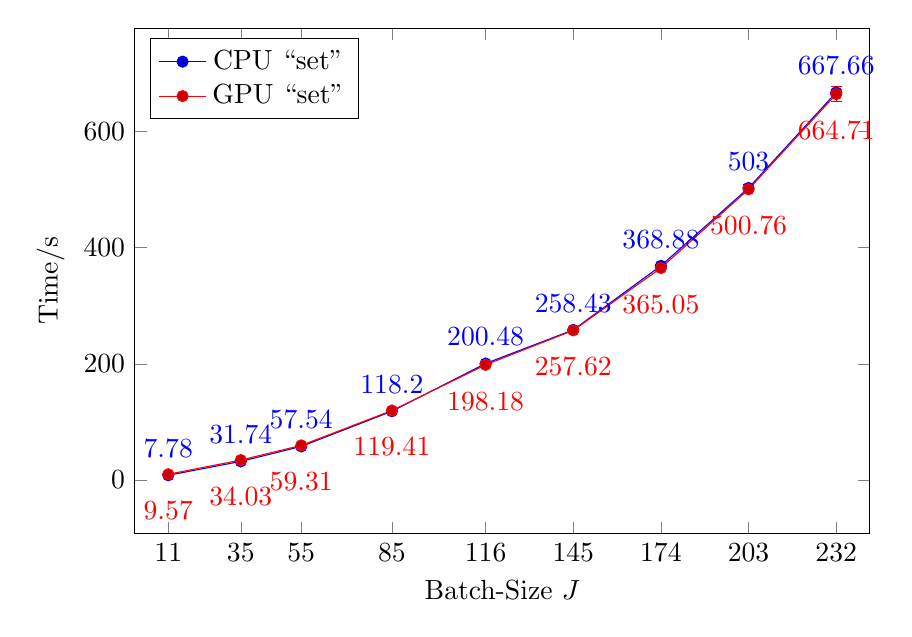
\begin{tikzpicture}
        \begin{axis}[
        width=.9\textwidth,
        height=8cm,
        xtick=data,
        xlabel={Batch-Size $J$},
        ylabel={Time/s},
        enlarge y limits=0.15,
        enlarge x limits=0.05,
        y tick label style={/pgf/number format/1000 sep=},
        extra y tick style={grid=major, tick label style={xshift=-1cm}},
        legend style={at={(0.02,.98)},
            anchor=north west},
        nodes near coords,
        every node near coord/.append style={yshift=-0.7cm}
        ]
        \addplot+ [mark=*,
        nodes near coords=\raisebox{0.8cm}{\pgfmathprintnumber\pgfplotspointmeta},error bars/.cd, y dir=both,y explicit
        ] coordinates {
            (11,7.78) +- (0.03,0.03)
            (35,31.74) +- (0.32,0.32)
            (55,57.54) +- (0.14,0.14)
            (85,118.20) +- (0.52,0.52)
            (116,200.48) +- (0.78,0.78)
            (145,258.43) +- (2.67,2.67)
            (174,368.88) +- (1.71,1.71)
            (203,503.00) +- (6.22,6.22)
            (232,667.66) +- (5.78,5.78)
        };  % cpu
        \addplot+ [mark=*,error bars/.cd, y dir=both,y explicit] coordinates {
            (11,9.57) +- (0.03,0.03)
            (35,34.03) +- (0.31,0.31)
            (55,59.31) +- (0.14,0.14)
            (85,119.41) +- (0.47,0.47)
            (116,198.18) +- (2.04,2.04)
            (145,257.62) +- (2.68,2.68)
            (174,365.05) +- (3.55,3.55)
            (203,500.76) +- (3.22,3.22)
            (232,664.71) +- (13.16,13.16)
        };  % gpu
        \legend{CPU ``set'',GPU ``set''}
        \end{axis}
        \end{tikzpicture}
        \caption{Time Taken by the Full Model: GPU Speedup over all batch-sizes is only $\textbf{0.97}\pm\textbf{0.04}$ - heavily impacted by LP runtimes.}
        \label{fig:Restricted Finding Rewards - Time Taken by the Full Model}
    \end{subfigure}\vspace*{1em}
    \begin{subfigure}{\textwidth}
        \centering
        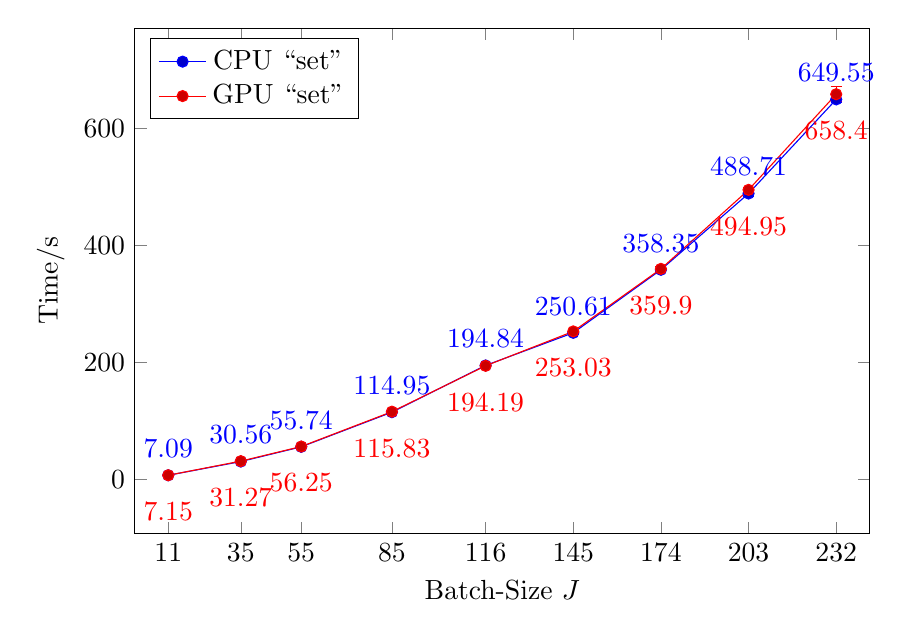
\begin{tikzpicture}
        \begin{axis}[
        width=.9\textwidth,
        height=8cm,
        xtick=data,
        enlarge y limits=0.15,
        enlarge x limits=0.05,
        xlabel={Batch-Size $J$},
        ylabel={Time/s},
        y tick label style={/pgf/number format/1000 sep=},
        legend style={at={(0.02,.98)},
            anchor=north west},
        nodes near coords,
        every node near coord/.append style={yshift=-0.7cm}
        ]
        \addplot+ [mark=*,
        nodes near coords=\raisebox{0.8cm}{\pgfmathprintnumber\pgfplotspointmeta},error bars/.cd, y dir=both,y explicit
        ] coordinates {
            (11,7.09) +- (0.04,0.04)
            (35,30.56) +- (0.32,0.32)
            (55,55.74) +- (0.14,0.14)
            (85,114.95) +- (0.49,0.49)
            (116,194.84) +- (0.84,0.84)
            (145,250.61) +- (2.47,2.47)
            (174,358.35) +- (1.68,1.68)
            (203,488.71) +- (5.74,5.74)
            (232,649.55) +- (5.93,5.93)
        };  % cpu
        \addplot+ [mark=*,error bars/.cd, y dir=both,y explicit] coordinates {
            (11,7.15) +- (0.04,0.04)
            (35,31.27) +- (0.30,0.30)
            (55,56.25) +- (0.13,0.13)
            (85,115.83) +- (0.47,0.47)
            (116,194.19) +- (2.03,2.03)
            (145,253.03) +- (2.67,2.67)
            (174,359.90) +- (3.57,3.57)
            (203,494.95) +- (3.20,3.20)
            (232,658.40) +- (13.15,13.15)
        };  % gpu
        \legend{CPU ``set'',GPU ``set''}
        \end{axis}
        \end{tikzpicture}
        \caption[Time taken by the LP]{Time taken by the LP: GPU Speedup over all batch-sizes is only $\textbf{0.99}\pm\textbf{0.005}$. Expectedly, there is no GPU Speedup in LP runtimes.}
        \label{fig:Restricted Finding Rewards - Time taken by the LP}
    \end{subfigure}
\end{figure}

\begin{figure}[!htbp]
    \centering
    \ContinuedFloat
    \begin{subfigure}{\textwidth}
        \centering
        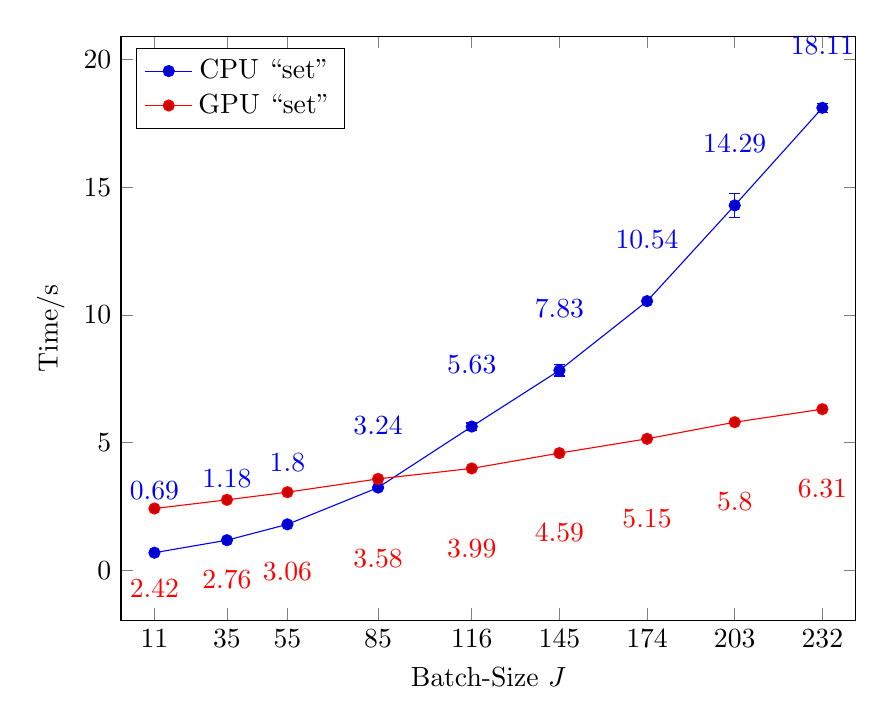
\begin{tikzpicture}
        \begin{axis}[
        width=.9\textwidth,
        height=9cm,
        xtick=data,
        enlarge y limits=0.15,
        enlarge x limits=0.05,
        xlabel={Batch-Size $J$},
        ylabel={Time/s},
        legend style={at={(0.02,.98)},
            anchor=north west},
        nodes near coords,
        every node near coord/.append style={yshift=-1.25cm}
        ]
        \addplot+ [mark=*,
        nodes near coords=\raisebox{1.8cm}{\pgfmathprintnumber\pgfplotspointmeta},error bars/.cd, y dir=both,y explicit] coordinates {
            (11,0.69) +- (0.004,0.004)
            (35,1.18) +- (0.002,0.002)
            (55,1.80) +- (0.01,0.01)
            (85,3.24) +- (0.03,0.03)
            (116,5.63) +- (0.14,0.14)
            (145,7.83) +- (0.22,0.22)
            (174,10.54) +- (0.03,0.03)
            (203,14.29) +- (0.48,0.48)
            (232,18.11) +- (0.17,0.17)
        };  % cpu
        \addplot+ [mark=*, error bars/.cd, y dir=both,y explicit] coordinates {
            (11,2.42) +- (0.01,0.01)
            (35,2.76) +- (0.01,0.01)
            (55,3.06) +- (0.01, 0.01)
            (85,3.58) +- (0.01,0.01)
            (116,3.99) +- (0.01,0.01)
            (145,4.59) +- (0.01,0.01)
            (174,5.15) +- (0.02,0.02)
            (203,5.80) +- (0.02,0.02)
            (232,6.31) +- (0.005,0.005)
        };  % gpu
        \legend{CPU ``set'',GPU ``set''}
        \end{axis}
        \end{tikzpicture}
        \caption{Time taken by the Neural Network: GPU Speedup over all batch-sizes is $\textbf{1.41}\pm\textbf{0.76}$ - as transfer time between RAM and GPU's internal memory dominates for smaller datasets. However, as batch-size increases, computation time dominates over transfer time - GPU ``set'' performs better than CPU ``set''.}
        \label{fig:Restricted Finding Rewards - Time taken by the Neural Network}
    \end{subfigure}\vspace*{1em}
    \begin{subfigure}{0.3\textwidth}
        \centering
        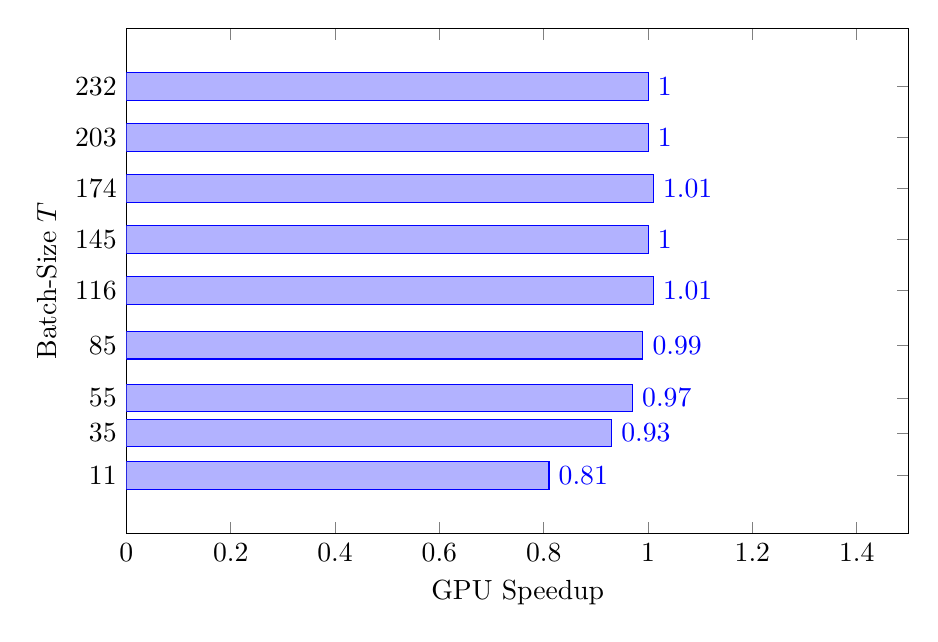
\begin{tikzpicture}
        \begin{axis}[
        xbar,
        width=0.95\textwidth,
        height=8cm,
        ytick=data,
        ylabel={Batch-Size $T$},
        xlabel={GPU Speedup},
        ytick align=inside,
        xmin=0,
        xmax=1.5,
        enlarge y limits=0.15,
        nodes near coords,
        ]
        \addplot+ coordinates {
            (0.81,11)
            (0.93,35)
            (0.97,55)
            (0.99,85)
            (1.01,116)
            (1.00,145)
            (1.01,174)
            (1.00,203)
            (1.00,232)
        };
        \end{axis}
        \end{tikzpicture}
        \caption{Speedup for the Full Model}
        \label{fig:Restricted Finding Rewards - Speedup for the Full Model}
    \end{subfigure}\hfill
    \begin{subfigure}{0.3\textwidth}
        \centering
        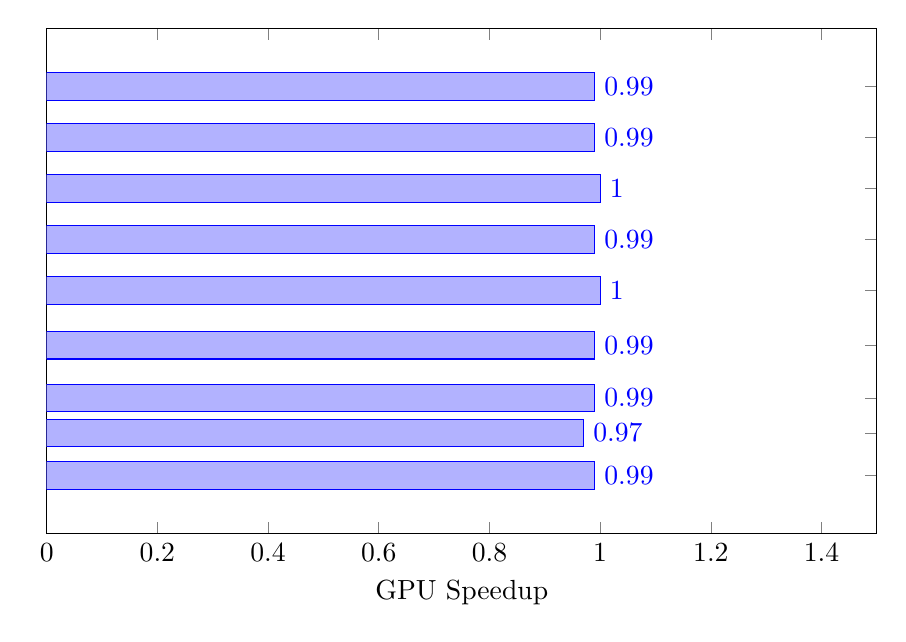
\begin{tikzpicture}
        \begin{axis}[
        xbar,
        width=\textwidth,
        height=8cm,
        ytick=data,
        yticklabels={,,},
        xlabel={GPU Speedup},
        ytick align=inside,
        xmin=0,
        xmax=1.5,
        enlarge y limits=0.15,
        nodes near coords,
        ]
        \addplot+ coordinates {
            (0.99,11)
            (0.97,35)
            (0.99,55)
            (0.99,85)
            (1.00,116)
            (0.99,145)
            (1.00,174)
            (0.99,203)
            (0.99,232)
        };
        \end{axis}
        \end{tikzpicture}
        \caption{Speedup for LP}
        \label{fig:Restricted Finding Rewards - Speedup for LP}
    \end{subfigure}\hfill
    \begin{subfigure}{0.4\textwidth}
        \centering
        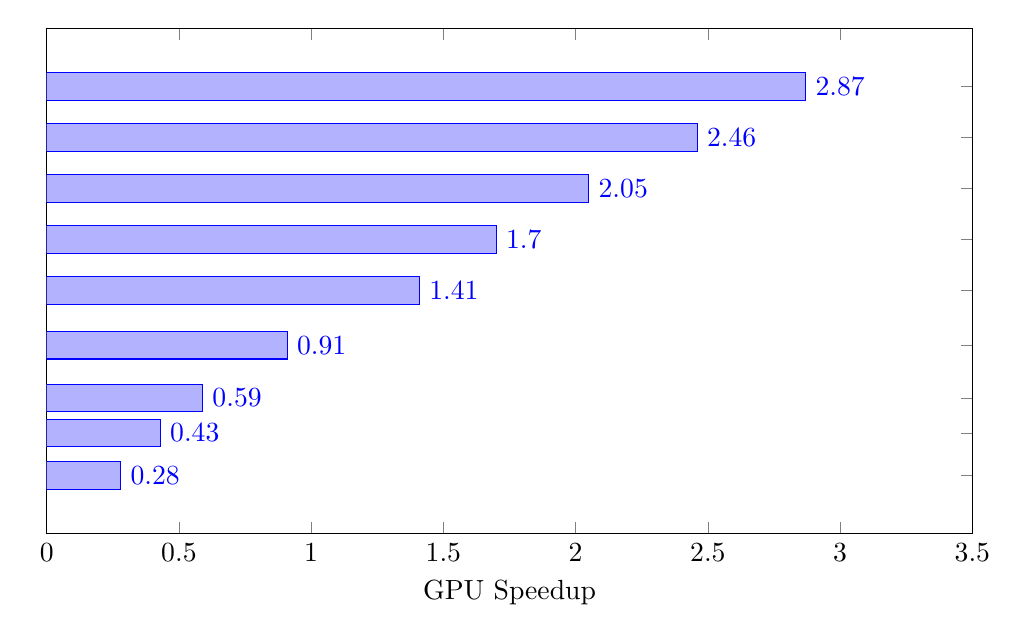
\begin{tikzpicture}
        \begin{axis}[
        xbar,
        width=1.1\textwidth,
        height=8cm,
        ytick=data,
        yticklabels={,,},
        xlabel={GPU Speedup},
        ytick align=inside,
        xmin=0,
        xmax=3.5,
        enlarge y limits=0.15,
        nodes near coords,
        ]
        \addplot+ coordinates {
            (0.28,11)
            (0.43,35)
            (0.59,55)
            (0.91,85)
            (1.41,116)
            (1.70,145)
            (2.05,174)
            (2.46,203)
            (2.87,232)
        };
        \end{axis}
        \end{tikzpicture}
        \caption{Speedup for the Neural Network}
        \label{fig:Restricted Finding Rewards - Speedup for the Neural Network}
    \end{subfigure}
    \caption[Finding Rewards After Restricing Script's Access to CPU Cores - Execution Times of Different Batch-Sizes $J$ with GPU and CPU ``set'' Separately]{Finding Rewards After Restricing Script's Access to CPU Cores - Execution Times of Different Batch-Sizes $J$ with GPU and CPU ``set'' Separately: Scaling is strongly hampered by the LP solver. Comparing the contributions of LP and Neural Network to total runtime on GPU ``set'', LP accounts for $\textbf{94.57}\pm\textbf{5.01}\%$ of the total time.}
    \label{fig:Restricted Finding Rewards - Execution Times of Different Batch-Sizes J with GPU and CPUa ``set'' Separately}
\end{figure}

\subsubsection{Final Results}
The results after restricting script's access to a single CPU cores are plotted in \Cref{fig:Restricted Finding Rewards - Execution Times of Different Batch-Sizes J with GPU and CPUa ``set'' Separately}. We prefer using these results (over previous results - \Cref{fig:Finding Rewards - Execution Times of Different Batch-Sizes J with GPU and CPU ``set'' Separately}) after restricting access, as it gives the better performance for CPU ``set''. The time elapsed for the Neural Network includes time taken to transfer tensors to and from the GPU, which results in overhead - as seen in higher runtimes for smaller datasets (lower batch-size) in \Cref{fig:Restricted Finding Rewards - Time taken by the Neural Network,fig:Restricted Finding Rewards - Speedup for the Neural Network}. However, as the batch-size increases, we see the computation dominating over the transfer time, resulting in higher CPU ``set'' runtimes; the GPU ``set'' runtimes almost grow linearly for the tested batch-sizes.

Moreover, the LP subproblem highly impacts the full model, accounting for more than $90\%$ of the total runtime. Therefore, even though the Neural Network gets sped up at bigger datasets, the GPU Speedup is not reflected in the full model.
    \chapter{Conclusion} \label{sec:Conclusion}
Our models for the Identification and the Pricing Problem outperformed previously studied ones \cite{Xue2016Avi2} and other baseline comparisons (\Cref{sec:IdProbRes - Optimization,sec:PriProbRes - Optimization,tab:Loss Values Calculated for Different Models for Identification Problem,tab:Loss Values Calculated from Different Sets of Rewards}). For the Identification Problem, the average loss value was $14\%$ lower than the previous 2-layered model, and $12\%$ better than the 4-layered model, giving us better results than any other tested model. While we did not test deeper networks, we contend that using more hidden layers will only aggravate overfitting and won't provide better results - as is partly the case with the 4-layered network. The Pricing Problem's model also delivered at least $3\times$~lower loss values than other baseline comparisons for reward distribution.

On the other hand, we can definitively conclude that the Identification Problem ran $\approx 9\times$~faster on the GPU than the CPU, mainly because the model was based on tensors and a neural network, accelerated by a GPU and NVIDIA's APIs. With an approximate GPU Speedup of $9.06$ for the Identification Problem, we can scale to large datasets more efficiently on the GPU than the CPU. The Pricing Problem's neural network only performed better with higher batch-sizes, with transfer times hampering performance on smaller datasets. Although the Pricing Problem's full model did not deliver a noticeable speedup (with the LP problem heavily impacting the runtime), the 2-layered network for finding rewards gave a speedup of $1.41\pm0.76$ (mean over all tested batch-sizes). This shows that neural network are inherently quick to optimize on a GPU only if the batch-sizes are large enough. This issue of high transfer times is also discussed in \Cref{sec:Computation Using GPUs} and recent literature \cite[Appendix~B]{PattersonARM}, inferring that one can witness GPU Speedups only when transfer time are tiny compared to computation time. Using faster GPUs like NVIDIA Quadro GP100, and those based on the newer Volta architecture will most likely decrease the models' runtimes. There still exists enormous scope for improvement on both fronts -- optimized results and faster computation.

\section{Interesting Inferences}
One may also notice compelling reflections from the results:
\begin{itemize}
    \item One interesting observation in \Cref{tab:Loss Values Calculated from Different Sets of Rewards} is that the loss value from the Proportional Distribution ($0.0235\%$) and Random Initialization ($0.0331\%$) are very close, highlighting that the set of weights obtained from the Identification Problem are dependent on other factors ($\matr{f}, \matr{D}$) as well. In other words, only incentivizing under-sampled locations more is as good as random distribution of rewards -- as agents consider environmental features and distances between locations to make decisions as well.
    
    \item By looking at the model's generated rewards (\Cref{tab:Example Rewards Prediction by the Pricing Problem's Model}), one can infer that the model chooses to place large rewards in very under-sampled locations, rather than distributing more evenly over all locations. Although this non-uniform distribution is unintuitive to the human perspective, it gives much lower results than proportionally allocated rewards.
    
    \item Algorithms that use different libraries for sub-routines' implementation can have difficulty in parallelizing. As we saw with the unexpected GPU Speedup in LP runtimes in the Pricing Problem (\Cref{sec:PriProbRes - GPU,app:GPU Speedup in LP Computation}), na\"ive synchronization barriers can affect performance in CPUs' multi-threading mechanism as well as GPUs' threads, if the logic requires branching (\Cref{sec:Avoiding Specific Operations in GPUs}). Therefore, one might consider threading the \textit{full} algorithm instead of using external libraries for threading some sub-routines.
    
    \item GPUs are not always effective in executing all kinds of models. Factors that affect the performance include the size of the model and datasets, extent of conditional statements in the program, requirement of synchronization barriers, data transfer between RAM and GPU, algorithm's `parallel-friendliness' and many more. Reducing model complexity always helps, but when the models are increasingly simple and small, CPUs can do a much better job than GPUs.
\end{itemize}
\begin{table}[!htbp]
    \centering
    \caption[Example Rewards Prediction by the Pricing Problem's Model]{Example Rewards Prediction by the Pricing Problem's Model: The prediction is relatively sparse and non-uniform. Parameters: $\mathcal{R} = 1000$, Loss value = $0.0068\%$, Epochs = 1000, Learning Rate = $5 \times 10^{-5}$, Weights: Set-2. (values rounded)}
    \label{tab:Example Rewards Prediction by the Pricing Problem's Model}
    \setlength\tabcolsep{2pt}
    \begin{tabular}{|*{15}{c}|}
        \hline
        0.00 & 38.02 & 0.00 & 0.00 & 0.00 & 0.00 & 14.12 & 0.00 & 24.63 & 4.43 & 3.18 & 24.35 & 0.00 & 19.53 & 0.00\\
        1.63 & 6.40 & 0.00 & 0.00 & 0.00 & 36.31 & 31.15 & 0.00 & 0.00 & 29.16 & 2.22 & 6.02 & 23.12 & 0.00 & 16.42\\
        0.00 & 0.00 & 28.45 & 0.00 & 37.50 & 0.00 & 20.04 & 34.19 & 0.00 & 0.00 & 18.29 & 0.00 & 0.00 & 21.33 & 0.00\\
        0.00 & 23.73 & 24.77 & 0.00 & 23.18 & 1.75 & 0.00 & 20.78 & 22.60 & 0.00 & 0.00 & 0.00 & 0.00 & 0.00 & 4.79\\
        4.67 & 0.00 & 0.00 & 34.82 & 0.00 & 9.47 & 0.00 & 0.00 & 31.43 & 0.00 & 4.35 & 16.55 & 28.51 & 6.02 & 0.00\\
        21.24 & 21.38 & 0.00 & 22.95 & 27.17 & 21.44 & 24.16 & 21.07 & 0.00 & 0.00 & 25.48 & 0.00 & 0.00 & 0.00 & 2.59\\
        12.28 & 0.00 & 0.00 & 0.00 & 0.00 & 0.00 & 22.09 & 0.00 & 0.00 & 16.50 & 0.00 & 2.88 & 1.57 & 0.00 & 43.45\\
        0.00 & 0.00 & 15.25 & 0.02 & 0.00 & 0.00 & 0.00 & 0.00 & 0.18 & 0.32 & 0.00&&&&\\ \hline
    \end{tabular}
\end{table}

\section{Limitations} \label{sec:Limitations}
We could not parallelize some sub-routines of \Cref{alg:Algorithm for the Identification Problem,alg:Solving the Pricing Problem} and had to rely on PyTorch's implementation for the most part. While PyTorch's implementation \cite{PTDocs} may be very efficient, we do not know if it suits our models best -- a typical problem when using external libraries.

On the other hand, we did not venture in adjusting the model's parameters much as the models took long time to tests, and there lied multiple possibilities. Tinkering with the models' characteristics might have optimized the models more if we had devised a way to experiment efficiently. This also remains a topic for future study.

We also could not venture in-depth of quirky behavior and ascertain reasons with high confidence. Our research project limited us to focus on improving the Avicaching game, restricting available time to rigorously study thread synchronization delays and GPU's architecture.

\section{Further Research}
There exist numerous possibilities for solving the problems better and faster -- from more complex models to better preprocessing to more parallel algorithms with fewer synchronization barriers. Some important suggestions are listed below:

\subsubsection{Choice of Gradient-Descent Algorithm}
\Cref{fig:Plot for 3-layered Model} shows how the choice of Adam's algorithm \cite{Adam} for \textsc{Gradient-Descent}($\cdot$) helps the model to learn quickly. However, we also witness long periods of saturation after a few epochs. This was the case for several other algorithms (SGD \cite{SGD} and Adagrad \cite{Adagrad}) as well, but with different paces of learning. Since the organizers would want to further optimize the set of weights, research could be done on avoiding the long, unwavering saturation phase. This may involve using other algorithms for \textsc{Gradient-Descent}($\cdot$) (\Cref{alg:Algorithm for the Identification Problem}) and/or altering the loss function ($Z_P$ -- \Cref{eqn:iden_problem}).

\subsubsection{Modeling LP Differently to Reduce Runtimes}
LP is a simple tool for optimizing different problems, with various algorithms for solving LPs - Simplex, Criss-Cross and other Interior Point techniques. While it gives optimal results, it can be computationally expensive if the matrices are large (as depicted in \Cref{fig:Restricted Finding Rewards - Time taken by the LP}). One can try several approaches to reduce computation time here:
\begin{itemize}
    \item Implement GPU or OpenMP backend for the LP.
    \item Constrain Rewards differently (\Cref{sec:Constraining Rewards}). Parallelized algorithms for constraining rewards can decrease the runtime for the Pricing Problem's model considerably as the current LP accounts for $\approx 94\%$ of the total runtime.
\end{itemize}


    \bibliographystyle{IEEEtran}
    \bibliography{IEEEabrv,avicaching}
    
    \cleardoublepage
    \begin{appendices}
    \crefalias{section}{appsec}
    \section{Implementation} \label{app:Implementation}
    The code can be found here[]. \\
    Both the Identification and the Pricing Problem were programmed in Python 2.7 using NumPy 1.12.1, SciPy 0.19.1 and Pytorch 0.1.12 modules [web cites] \cite{SCPOptimizeDocs}\cite{NPDocs}. [Results from Python plotted in Matplotlib 2.0.2] With some code optimizations, the input dataset $\matr{F}$ was built using NumPy's \texttt{ndarray} and Pytorch's \texttt{tensor} functions. Since Pytorch offers NumPy-like code base but with dedicated neural network functions and submodules, Pytorch's \texttt{relu} and \texttt{softmax} functions were used along with other matrix operations.\\
    
    \subsection{Specific Implementation Details for the Pricing Problem}
    Among all the code optimizations in both models, some in that for the Pricing Problem are worth discussing, as they drastically differ from Algorithm \ref{alg:Solving the Pricing Problem} or are intricate. Most optimizations relevant to the Identification Problem are trivial and relate directly to those for the Pricing Problem. Therefore, only those in the Pricing Problem model are discussed.
    
    \subsubsection{Building the Dataset $\matr{F}$}
    Notice that we build the dataset $\matr{F}$ and batch-multiply it with $\matr{w_1}$ on each iteration/epoch (lines 2-3 of Algorithm \ref{alg:Solving the Pricing Problem}). Doing these steps are repetitive as most elements of $\matr{F}$, distances $\matr{D}$ and environmental feature vector $\vect{f}$, do not change unlike rewards $\vect{r}$. Moreover since $\matr{w_1}$ is fixed, Algorithm \ref{alg:Solving the Pricing Problem} would repetitively multiply the $\vect{f}$ and $\matr{D}$ components of $\matr{F}$ with $\matr{w_1}$. To avoid these unnecessary computations, we preprocessed most of $\matr{F}$ by batch-multiplying with $\matr{w_1}$ and only multiplied $\vect{r}$ with the corresponding elements of $\matr{w_1}$. Figure \ref{fig:Splitting and Batch Multiplying F and w1} describes the process graphically.\\
    \begin{figure}[!htbp]
        \centering
        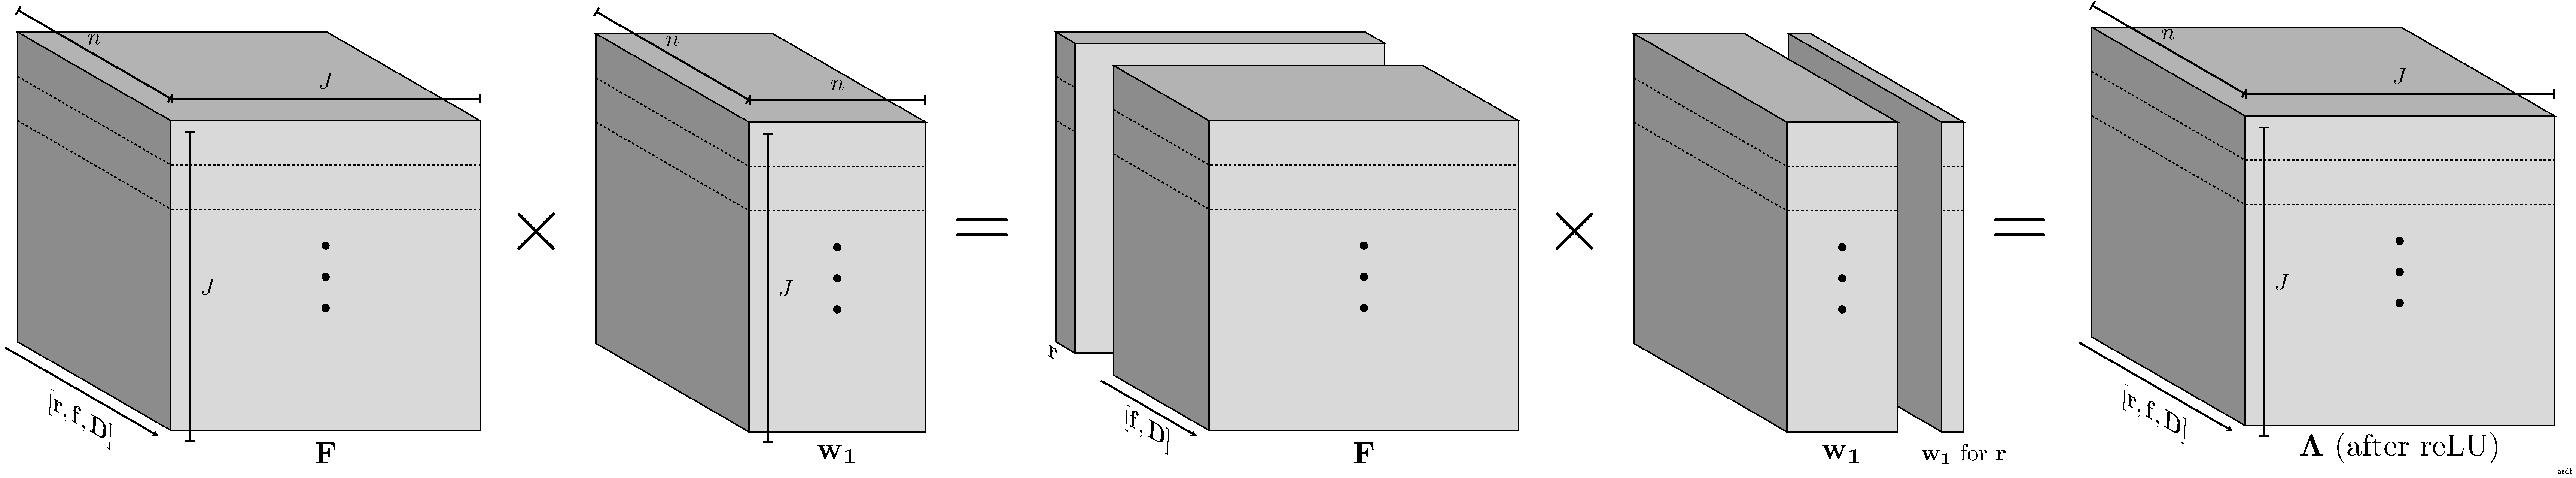
\includegraphics[width=\linewidth]{split_and_batch_multiply}
        \caption{Splitting and Batch Multiplying $\matr{F}$ and $\matr{w_1}$}
        \label{fig:Splitting and Batch Multiplying F and w1}
    \end{figure}    
    Although this preprocessing might seem applicable for the model in Identification Problem too, it does not apply fully. Since the weights $\matr{w_1}$ are updated on each iteration/epoch, we cannot multiply them with parts of $\matr{F}$ beforehand (Algorithm \ref{alg:Algorithm for the Identification Problem}). However, we can combine $\matr{D}$ and $\vect{f}$ in the preprocessing stage and simply append $\vect{r}[t]$ on each iteration, saving computation time.
    
    \subsubsection{Modeling the Linear Programming Problem in the Standard Format}
    The \texttt{scipy.optimize} module's \texttt{linprog} function requires that the arguments are in standard LP format. As discussed in \cref{sec:Calculating Rewards}, Equation \ref{eqn:lp_code_constrain_rewards} resembles the standard format more closely than \ref{eqn:lp_math_constrain_rewards}, but it may not be clear how so.\\
    
    Considering $\vect{u}$ and $\vect{r'}$ as variables $\vect{x}$, Equation \ref{eqn:lp_code_constrain_rewards} translates into Equation \ref{eqn:lp_matrix_rewards} ($J$ is the number of locations).
    \begin{equation} \label{eqn:lp_matrix_rewards}
    \begin{aligned}
    & \text{minimize}
    & & \begin{bmatrix}
    \vect{0_J}\\
    \vect{1_J}\\
    \end{bmatrix}^T
    \begin{bmatrix}
    \vect{r'}\\
    \vect{u}
    \end{bmatrix}\\ \\
    & \text{subject to}
    & & \begin{bmatrix}
    I_J & -I_J\\
    -I_J & -I_J\\
    \vect{1}^T_J & \vect{0}^T_J\\
    \end{bmatrix}
    \begin{bmatrix}
    \vect{r'}\\
    \vect{u}\\
    \end{bmatrix} \leq
    \begin{bmatrix}
    \vect{r}\\
    -\vect{r}\\
    \mathcal{R}\\
    \end{bmatrix}\\
    &&& r'_i, u_i \geq 0
    \end{aligned}
    \end{equation}
    
    \section{Strange GPU Speedup in LP Computation} \label{app:Strange GPU Speedup in LP Computation}
    Even though we intentionally transferred the rewards vector to and constrained it using \texttt{scipy.optimize} module's \texttt{linprog} function on the CPU, we obtained an unexpected GPU Speedup in the LP runtimes (see \cref{sec:PriProbRes - GPU} and Figure \ref{fig:Finding Rewards - Time taken by the LP}). Confounded by this weird behavior, we wanted to pinpoint the reason(s) because SciPy's function could not have differentiated between the configurations and delivered different results. However, since this was not our research's prime motive, we did not take a strong quantitative approach in determining the cause(s).
    
    \subsection{Possible Reasons for GPU Speedup} \label{app:Possible Reasons for GPU Speedup}
    There could have been many reasons for this bizarre behavior, including but not limited to:
    \begin{enumerate}
        \item SciPy's Optimize Module differentiating between configurations. This can be ruled out because the module could not have known the configuration during which it was called. This is because the configuration settings were applicable only on user-programmed operations, and needed to be explicitly stated - as mandated by Pytorch \cite{PTDocs}. SciPy's Optimize Module identifying the configurations is just supernatural.
        \item CPU ``set'' using exploiting more main memory than GPU ``set''. We suspected that since CPU ``set'' configuration's operations were executed solely on the CPU, the residing datasets could have used more main memory than when GPU ``set'' was running. This could have hampered the performance of LP with CPU ``set'', as the LP had lesser space to operate in. Unlike the 1\textsuperscript{st} possibility, this would have meant that CPU ``set'' was slowing down the LP, and not that GPU ``set'' was speeding up the LP.
        \item Neural network in CPU ``set'' using more CPU threads than that in GPU ``set''. The Intel i7-7700K processor is quad-core with 8 threads. Since Pytorch uses OpenMP \cite{PTDocs}, a parallel processing API for CPUs, we fancied the neural network to utilize more threads than that in GPU ``set'', thus allowing less available threads for the LP to run. 
        
        However, given that our scripts in Python did not explicitly use parallel programming with CPU ``set'' and the code was sequential, one could very well suggest that upon completion of the neural network, all threads should have been synchronized, after which the LP would have started. This would have meant that the LP's resources would have been independent of the neural network's resources, raising questions on this possibility.
    \end{enumerate}

    \subsection{LP Slowing Down or Speeding Up?} \label{app:LP Slowing Down or Speeding Up?}
    First we determined whether the LP runtime was being sped up with GPU ``set'' or slowed down with CPU ``set''. To test this, we created a copy of our Pricing Problem's model, which focused only on logging LP runtimes at each epoch. For a baseline comparison, we scripted the same LP \textit{without} the neural network, which gave us the \underline{original} runtimes for the LP (ran for equal number of epochs), without any involvement of Pytorch modules or functions. 
    
    Comparing the former runtimes (CPU and GPU ``set'') with `Only LP' runtime (independent script) in Figure \ref{fig:LP Runtime Example for Different Configurations}, we observed that the LP in the CPU ``set'' configuration took longer to execute than that in  `Only LP' setting during each epoch. We also noticed little to no interaction between the neural network in GPU ``set'' with the LP, as the runtimes of LP in GPU ``set'' were similar to those of LP in `Only LP' setting. This confirmed that CPU ``set'' was slowing down the LP and GPU ``set'' was not speeding it up. But why?
    \begin{figure}[!htbp]
        \centering
        \begin{tikzpicture}
        \begin{axis}[
            width=\textwidth,
            height=8cm,
            xlabel=Epochs,
            ylabel=Time/s,
            scaled y ticks = false,
            grid=both,
            every axis plot/.append style={very thick},
        ]
        \addplot[red] table [col sep=comma,x=epoch, y=cpuset]{datafiles/lp_time_logs.csv};
        \addlegendentry{CPU ``set''}
        
        \addplot[blue] table [col sep=comma,x=epoch, y=gpuset]{datafiles/lp_time_logs.csv};
        \addlegendentry{GPU ``set''}
        
        \addplot[brown] table [col sep=comma,x=epoch, y=onlylp]{datafiles/lp_time_logs.csv};
        \addlegendentry{`Only LP'}
        
        \end{axis}
        \end{tikzpicture}
        \caption[LP Runtime Example for Different Configurations]{LP Runtime Example for Different Configurations: LPs in both CPU and GPU ``set'' start running slowly, but pick up speed after $\approx$ 20 epochs. We could not explain the presence of spikes in LP runtimes of CPU ``set'' and their absence in GPU ``set''. The test was done on a random dataset for 200 epochs, while the other experiment specifications were same as in \cref{sec:Experiment Specifications}.}
        \label{fig:LP Runtime Example for Different Configurations}
    \end{figure}
    
    \subsection{CPU and Main Memory Usage} \label{app:CPU and Main Memory Usage}
    While logging the LP runtimes in \cref{sec:LP Slowing Down or Speeding Up?}, we also recorded an estimate of the amount of computer resources both configurations were using. Using the \texttt{top} package in Ubuntu, we polled the resource monitor every 0.1 seconds while the python script was running\footnote{\label{foo:logs not epochs} Running processes were polled every 0.1 seconds - contributing to a `log'. The longer the script ran, the more logs collected.}. Figures \ref{fig:CPU Usage by Different Configurations} and \ref{fig:Main Memory Usage by Different Configurations} shows how much main memory and CPU resource each setting was using.
    
    It is fascinating to see that CPU ``set'' constantly used more than 4 out of 8 available threads, i.e., $>400\%$ CPU usage, during execution, while GPU ``set'' only used a single thread. Also, since we polled at every 0.1 second, and the LP took a minimum of 0.14 seconds (Figure \ref{fig:LP Runtime Example for Different Configurations}), the data displayed in Figure \ref{fig:CPU Usage by Different Configurations} must show resource use \textit{while} the LP was running. Considering that the LP in `Only LP' setting only used a single thread (100\%), it makes sense that GPU ``set'' would use 1 thread for execution - the neural network operations were performed on the GPU, leaving the CPU empty for management and LP. On the other hand, it is apparent that CPU ``set'' had multi-threaded operations running simultaneously, even though we reasoned its low possibility (\#3 in \cref{sec:Possible Reasons for GPU Speedup}). Since we know from the `Only LP' setting that the LP only used a single thread, the other threads in CPU ``set'' must have been the neural network. Although this counters our reasoning that the neural network threads should have synchronized before the LP started, it seems that those threads were still active. While we cannot explain this behavior, this activity does not impact correctness, as found from optimization tests on CPU ``set''\footnote{CPU ``set'' tests were done for optimization on original datasets to check this. Since we got the same results as for GPU ``set'' optimization tests \cref{sec:PriProbRes - Optimization}, the results are not shown in the report.} (same optimization figures as obtained for GPU ``set'' - \cref{sec:PriProbRes - Optimization}).
    
    On the other hand, GPU ``set'' was using 10 times as much main memory as CPU ``set'' or `Only LP', even though all matrix operations were executed and stored on the GPU. Not only this is weird, but it is also opposite of what we expected to happen - CPU ``set'' using more main memory and hampering LP performance. It is ironic that the LP performs better (even as good as `Only LP') on GPU ``set'' even when the configuration uses a lot more main memory than CPU ``set''. Clearly, the main memory usage cannot be a criterion for assessing LP performance on different configurations.
    \begin{figure}[!htbp]
        \centering
        \begin{minipage}{.49\textwidth}
            \centering
            \begin{tikzpicture}
            \begin{axis}[
            name=cpuusage-cpuset,
            width=\textwidth,
            enlarge x limits=0.15,
            no markers,
            ymax=800,
            ymin=0,
            ]
            \addplot+[fill=red, opacity=.4] table [col sep=comma,x=epoch, y=cpu]{datafiles/ext_cpu_cpuset.csv} \closedcycle;
            
            \addplot+[very thick, red!50!black] table [col sep=comma,x=epoch, y=cpu]{datafiles/ext_cpu_cpuset.csv};
            
            \end{axis}
            
            \begin{axis}[
            name=cpuusage-gpuset,
            at=(cpuusage-cpuset.below south west), anchor=above north west,
            width=\textwidth,
            enlarge x limits=0.15,
            no markers,
            ylabel={CPU Usage/\%},
            ymax=200,
            ymin=0,
            ]
            \addplot+[fill=blue, opacity=.4] table [col sep=comma,x=epoch, y=cpu]{datafiles/ext_cpu_gpuset.csv} \closedcycle;
            
            \addplot+[very thick, blue!50!black] table [col sep=comma,x=epoch, y=cpu]{datafiles/ext_cpu_gpuset.csv};
            \end{axis}
            
            \begin{axis}[
            name=cpuusage-onlylp,
            at=(cpuusage-gpuset.below south west), anchor=above north west,
            width=\textwidth,
            enlarge x limits=0.15,
            no markers,
            xlabel={Logs},
            ymax=200,
            ymin=0,
            ]
            \addplot+[fill=green, opacity=.4] table [col sep=comma,x=epoch, y=cpu]{datafiles/ext_onlylp.csv} \closedcycle;
            
            \addplot+[very thick, green!50!black] table [col sep=comma,x=epoch, y=cpu]{datafiles/ext_onlylp.csv};
            \end{axis}
            \end{tikzpicture}
            \caption[CPU Usage by Different Configurations]{CPU Usage by Different Configurations\textsuperscript{\ref{foo:logs not epochs}}: From top - CPU ``set'', GPU ``set'', `Only LP'. CPU Usage for GPU ``set'' and `Only LP' are very similar as operations other than the LP run on the GPU.}
            \label{fig:CPU Usage by Different Configurations}
        \end{minipage}\hfill
        \begin{minipage}{.49\textwidth}
            \centering
            \begin{tikzpicture}
            \begin{axis}[
            name=memusage-cpuset,
            width=\textwidth,
            enlarge x limits=0.15,
            no markers,
            ymax=1,
            ymin=0,
            ]
            \addplot+[fill=red, opacity=.4] table [col sep=comma,x=epoch, y=mem]{datafiles/ext_cpu_cpuset.csv} \closedcycle;
            
            \addplot+[very thick, red!50!black] table [col sep=comma,x=epoch, y=mem]{datafiles/ext_cpu_cpuset.csv};
            
            \end{axis}
            
            \begin{axis}[
            name=memusage-gpuset,
            at=(memusage-cpuset.below south west), anchor=above north west,
            width=\textwidth,
            enlarge x limits=0.15,
            no markers,
            ylabel={Main Memory Usage/\%},
            ymax=10,
            ymin=0,
            ]
            \addplot+[fill=blue, opacity=.4] table [col sep=comma,x=epoch, y=mem]{datafiles/ext_cpu_gpuset.csv} \closedcycle;
            
            \addplot+[very thick, blue!50!black] table [col sep=comma,x=epoch, y=mem]{datafiles/ext_cpu_gpuset.csv};
            \end{axis}
            
            \begin{axis}[
            name=memusage-onlylp,
            at=(memusage-gpuset.below south west), anchor=above north west,
            width=\textwidth,
            enlarge x limits=0.15,
            no markers,
            xlabel={Logs},
            ymax=1,
            ymin=0,
            ]
            \addplot+[fill=green, opacity=.4] table [col sep=comma,x=epoch, y=mem]{datafiles/ext_onlylp.csv} \closedcycle;
            
            \addplot+[very thick, green!50!black] table [col sep=comma,x=epoch, y=mem]{datafiles/ext_onlylp.csv};
            \end{axis}
            \end{tikzpicture}
            \caption[Main Memory Usage by Different Configurations]{Main Memory Usage by Different Configurations\textsuperscript{\ref{foo:logs not epochs}}: From top - CPU ``set'', GPU ``set'', `Only LP'. The neural network doesn't occupy much main memory in CPU ``set'' - could be due to Python/Pytorch's garbage collection.}
            \label{fig:Main Memory Usage by Different Configurations}
        \end{minipage}
    \end{figure}

    \subsubsection{Inexplicable Behavior} \label{app:Inexplicable Behavior}
    The machine's resource logs while model execution defy our expectations starkly. Elaborated in \cref{sec:CPU and Main Memory Usage}, it is clear that Main Memory Usage does not explain the strange GPU Speedup in LP runtimes for CPU and GPU ``set''; instead, main memory logs show the opposite picture - with GPU ``set'' using $\approx$ 10 times as much main memory as CPU ``set'' or `Only LP'.
    
    On the other hand, CPU Usage logs do correspond with our LP runtime observations, but the former phenomenon is inexplicable, at least from our side. We believe that the neural network should stop executing and the threads should synchronize, before the LP starts. The LP on CPU ``set'' should then use just 1 thread, as with `Only LP' setting, forming high spikes in the CPU usage graph (top, Figure \ref{fig:CPU Usage by Different Configurations}). At odds with what we expect, the CPU Usage graph shows constant use of 4-5 threads with tiny spikes, which are natural, indicating that the neural network's threads were running \textit{along with} the LP. While this would have targeted the model's correctness on CPU ``set'' config., the results we obtained are same as those with GPU ``set''.
    
    Therefore, while CPU usage logs for the configurations might explain the strange GPU Speedup, CPU usage for CPU ``set'' is itself strange and inexplicable. Additionally, main memory usage in GPU ``set'' is inexplicably high. Although both these behaviors could be caused by Pytorch's implementation specifics, we cannot ensure this possibility. Further research and suggestions are welcome.
\end{appendices}
\end{document}